\documentclass[12pt]{article}

\usepackage{sbc-template}

\usepackage{graphicx,url}
\usepackage{subcaption}
\usepackage{float}

\usepackage[brazil]{babel}
\usepackage[utf8]{inputenc}  

%para tabelas mais complexas
\usepackage{tabularx}
\usepackage{booktabs}
\usepackage{caption}
\usepackage{amsmath}
\usepackage{amssymb}
\usepackage{threeparttable}

\usepackage[hidelinks]{hyperref}
     
\sloppy

\title{Caderneta Inteligente da Gestante: utilizando IA generativa com uma abordagem responsável para apoio ao
pré-natal}

\author{Lucas Zegrine Duarte\inst{1}, Humberto Torres Marques Neto\inst{1}}

\address{Instituto de Ciências Exatas e Informática\\
  Pontifícia Universidade Católica de Minas Gerais (PUC Minas)\\
  Caixa Postal 1.686, 30.535-901, Belo Horizonte, MG, Brazil
  \email{\{humberto.neto, lucas.duarte.1327493\}@sga.pucminas.br}
}

%%%%%%%%%%%%%%%%%%%%%%%%%%%%%%%%%%%%%%%%%%%%%%%%%%%%%%%%%%%%%%%%%%%%%%%%%%%%%%%%%%%%%%%%%%%%%%%%%%%%%%%%%%%%%%%%%%%%%%%%%%%%%%%%%%%%%%%%%%%%%%%%%%%%%%%%%%%%%%%%%%%%%%

\begin{document}

\maketitle

\begin{abstract}
  Prenatal documentation in Brazil is fragmented between physical and digital records, while the use of \textit{Large Language Models} in the public sector poses privacy and hallucination risks.
  This work proposes an \textit{on-premise} architecture integrating local voice transcription, \textit{Retrieval-Augmented Generation} over Ministry of Health manuals orchestrated via \textit{Ollama}, and a dedicated privacy gateway to mask PII before model inference.
  % To ensure clinical safety, a mandatory human-in-the-loop validation constraint is applied. The primary contribution is a secure and replicable high-fidelity prototype.
  Clinical safety is addressed through mandatory human-in-the-loop validation.
  The main contribution is a replicable high-fidelity prototype focused on privacy, auditability, and human review.
  The main limitation is the dependence on local hardware with high \textit{VRAM} capacity to support low-latency inference.
\end{abstract}

\begin{resumo}
  % A documentação de pré-natal no Brasil é fragmentada entre registros físicos e digitais, enquanto o uso de Modelos de Linguagem de Grande Escala no setor público levanta riscos de privacidade e alucinação.
  % Este trabalho propõe uma arquitetura \textit{on-premise} que integra transcrição de voz local, Geração Aumentada por Recuperação sobre manuais do Ministério da Saúde com orquestração via \textit{Ollama} e um gateway de privacidade dedicado para mascarar PII antes da inferência do modelo.
  % Para garantir a segurança clínica, exige-se revisão médica antes de salvar qualquer registro (\textit{human-in-the-loop}). A contribuição principal é a implementação de um protótipo de alta fidelidade replicável com foco em privacidade, auditabilidade e revisão humana.
  % A principal limitação é a dependência de hardware local com alta capacidade de \textit{VRAM} para suportar inferências com baixa latência.
  A documentação de pré-natal no Brasil é fragmentada entre registros físicos e digitais, enquanto o uso de \textit{LLMs} no setor público levanta riscos de privacidade e alucinação.
  Este trabalho propõe uma arquitetura \textit{on-premise} que integra transcrição de voz local, Geração Aumentada por Recuperação sobre manuais do Ministério da Saúde orquestrada via \textit{Ollama} e um gateway de privacidade para mascarar PII antes da inferência do modelo.
  A segurança clínica é tratada por meio de validação humana obrigatória.
  A principal contribuição é um protótipo de alta fidelidade replicável com foco em privacidade, auditabilidade e revisão humana.
  A principal limitação é a dependência de hardware local com alta capacidade de \textit{VRAM} para inferência com baixa latência.
\end{resumo}

\noindent \textbf{Palavras-chave:} Cuidado pré-natal; Inteligência artificial; Sistemas de informação em saúde; Privacidade de dados; Geração Aumentada por Recuperação; IA Explicável; Aplicações de LLM em saúde.

%%%%%%%%%%%%%%%%%%%%%%%%%%%%%%%%%%%%%%%%%%%%%%%%%%%%%%%%%%%%%%%%%%%%%%%%%%%%%%%%%%%%%%%%%%%%%%%%%%%%%%%%%%%%%%%%%%%%%%%%%%%%%%%%%%%%%%%%%%%%%%%%%%%%%%%%%%%%%%%%%%%%%%

\section{Introdução}

% A Inteligência Artificial (IA) tem demonstrado potencial transformador na saúde pública, oferecendo soluções para otimização de fluxos de trabalho e suporte à decisão \cite{Rajpurkar2022, Cabitza2022}.
% % No contexto do atendimento pré-natal, aplicações preditivas baseadas em aprendizado de máquina apontam potencial e desempenho promissor em bases experimentais na identificação precoce de riscos gestacionais \cite{HighRiskPregnancy2025, MachineLearning2022}.
% No contexto do atendimento pré-natal, estudos com bases reais de imagem e avaliação fetal têm explorado análises clínicas específicas, como a avaliação de expressões faciais associadas à dor fetal \cite{Rosa2020FetalPain, Bernardes2022FetalPain}, reforçando o interesse em soluções digitais aplicadas ao acompanhamento pré-natal.
% Contudo, a mortalidade e a morbidade materna no Brasil permanecem como desafios persistentes de saúde pública, associados a desigualdades no acesso à assistência pré-natal e à necessidade de correção dos dados oficiais sobre mortes maternas \cite{AcessoPreNatal2018, Laurenti2010}.

% A documentação clínica no \textit{Sistema Único de Saúde} (SUS) combina registros em sistemas digitais e instrumentos físicos independentes, como fichas de pré-natal e a Caderneta da Gestante \cite{FichaPreNatal2018, CadernetaGestante2024}.
% Essa fragmentação motiva a investigação de alternativas que apoiem o registro documental durante a consulta, sem substituir a validação profissional.

% Para atenuar essa sobrecarga, o presente trabalho propõe a especificação de uma plataforma digital \textit{on-premise} que integra transcrição de voz para texto (\textit{Speech-to-Text}) e agentes de IA baseados em \textit{Geração Aumentada por Recuperação} (RAG).
% A plataforma busca automatizar o preenchimento de formulários clínicos durante a consulta e apoiar o profissional, com base em protocolos oficiais do Ministério da Saúde, no cuidado com a paciente.

% %\subsection{Justificativa}
% % Justificativa
% %  - Depoimentos de profissionais de saúde sobre a solucao proposta e o cenario atual
% %  - Deve háver método para coletar depoimentos de profissionais de saúde sobre a solucao proposta e o cenario atual na landing page
% %  - Pode levar a necessidade de liberacao de comite de etica

% Complicações gestacionais e gravidez de alto risco demandam acompanhamento rigoroso.
% Segundo as diretrizes dos Manuais de Gestação de Alto Risco do Ministério da Saúde \cite{ManualAltoRisco2022, ManualAltoRisco2012}, condições de risco ou morbidades pré-existentes exigem estratificação contínua e acesso rápido a protocolos de acompanhamento.

% Para otimizar esse monitoramento e atenuar a sobrecarga informacional, modelos generativos têm sido progressivamente propostos como assistentes virtuais clínicos para resumo e triagem de dados \cite{Clusmann2023, Rajpurkar2022}.

% No entanto, a implantação irrestrita de Modelos de Linguagem de Grande Escala (LLMs) em cenários públicos de saúde depara-se com barreiras críticas: o risco de exposição de dados sensíveis (\textit{Personally Identifiable Information} -- PII), com potenciais implicações para a conformidade com a Lei Geral de Proteção de Dados (LGPD) \cite{OWASPLLM2025, LGPD2018}, e a propensão à geração de respostas não fundamentadas ou clinicamente inadequadas.

% Portanto, a justificativa técnica deste projeto fundamenta-se na estruturação de uma arquitetura local e auditável para apoio documental ao pré-natal, reduzindo a dependência de serviços externos no processamento de áudio e texto sensível.
% A proposta combina execução \textit{on-premise}, recuperação aumentada por documentos oficiais do Ministério da Saúde e revisão humana obrigatória, de modo que o modelo generativo não receba autonomia decisória nem persista informações sem validação profissional.

% A adoção de RAG busca reduzir o risco de respostas desvinculadas dos protocolos utilizados como base documental, embora não elimine a necessidade de avaliação de aderência e de revisão humana.
% De forma complementar, o gateway de privacidade aplica mecanismos de detecção e mascaramento de PII antes da inferência pelo modelo generativo, contribuindo para um fluxo mais controlável sob a perspectiva de privacidade por desenho, minimização de dados e auditabilidade.
% Assim, o foco do trabalho não é demonstrar eficácia assistencial, mas avaliar a viabilidade técnica, os limites e os trade-offs de uma arquitetura assistiva, local e não autônoma para o contexto do SUS.

% % Portanto, a justificativa técnica deste projeto fundamenta-se na necessidade de estruturar uma arquitetura que:
% % (i) assegure maior controle local sobre o ciclo de vida dos dados por meio de processamento local e isolado;
% % (ii) minimize o impacto das alucinações utilizando (\textit{RAG}) para ancorar o agente estritamente em protocolos de referência das cartilhas governamentais;
% % (iii) adote um \textit{gateway} de privacidade dedicado e um fluxo \textit{human-in-the-loop}, alinhado a princípios de supervisão humana efetiva, responsabilização, privacidade e proteção de dados em sistemas de IA no setor público \cite{FrameworkGovBR2025};
% % e (iv) incorpore mecanismos de detecção e mascaramento de \textit{PII} antes de submeter informações sensíveis aos modelos generativos.

% % Problema de Pesquisa

% A pesquisa baseia-se na seguinte pergunta norteadora: \textit{Como especificar, implementar e avaliar um protótipo 'on-premise' para apoio documental ao pré-natal a partir de protocolos públicos, sem atribuir autonomia decisória ao modelo generativo?}

% Para responder a este problema geral, as seguintes subquestões operacionais são investigadas:
% \begin{itemize}
%   \item Como estruturar uma arquitetura local em contêineres que reduza o risco de exposição de áudio ou dados textuais sensíveis?
%   \item Qual é o desempenho do módulo RAG na recuperação de documentos e trechos relevantes dos manuais oficiais de pré-natal?
% 	\item Qual é a aderência das respostas geradas por um LLM local aos critérios de protocolo de atendimento pré-natal no SUS?
% 	\item Em que medida um anonimizador de dados pessoais sensíveis mascara entidades antes da inferência pelo modelo generativo?
% 	\item Quais são os custos de latência associados à execução local do protótipo em comparação com uma linha de base externa?
% \end{itemize}

% % Objetivo Geral

% O objetivo geral deste projeto é especificar, implementar e avaliar uma plataforma digital \textit{on-premise} para apoio documental ao pré-natal, integrando um \textit{LLM} fundamentado via \textit{RAG} e mascaramento de PII para apoiar o registro documental e a consulta a protocolos de pré-natal, com ênfase em explicabilidade, privacidade por desenho, auditabilidade e alinhamento às diretrizes públicas de saúde.

% % Objetivos Específicos

% Para atingir o objetivo geral, delineiam-se os seguintes objetivos específicos:

% \begin{enumerate}
%   % \item Revisar a literatura sobre IA Responsável em saúde pública para fundamentar as decisões arquiteturais e delimitar a lacuna tecnológica no contexto do SUS;
%   % \item Dimensionar os requisitos de hardware e projetar uma topologia de rede \textit{on-premise} isolada em contêineres \textit{Docker};
%   \item Desenvolver um protótipo funcional voltado à consulta assistida de informações de pré-natal, mantendo revisão humana obrigatória;
%   \item Implementar um módulo de anonimização dedicado ao mascaramento e sanitização de PII brasileiras;
%   \item Estruturar a recuperação de conhecimento via (\textit{RAG}) com base em documentos públicos oficiais;
%   \item Avaliar o desempenho do protótipo por meio de métricas de recuperação, aderência automática de respostas em testes sintéticos e análise de latência.
%   \item Analisar os ganhos e perdas entre privacidade local, custo computacional, latência e viabilidade de implantação em ambientes de produção.
% \end{enumerate}

% O restante deste artigo está estruturado da seguinte forma: o referencial teórico embasa as decisões de design; os materiais e a metodologia detalham o ambiente e o fluxo de desenvolvimento; a solução proposta apresenta a arquitetura e interfaces criadas; e as seções finais discutem o desempenho e as limitações do ecossistema.

A Inteligência Artificial (IA) tem demonstrado potencial transformador na saúde pública, oferecendo soluções para otimização de fluxos de trabalho e suporte à decisão \cite{Rajpurkar2022, Cabitza2022}.
No contexto do atendimento pré-natal, estudos com bases reais de imagem e avaliação fetal têm explorado análises clínicas específicas, como a avaliação de expressões faciais associadas à dor fetal \cite{Bernardes2022FetalPain}, reforçando o interesse em soluções digitais aplicadas ao acompanhamento pré-natal.
Contudo, a mortalidade e a morbidade materna no Brasil permanecem como desafios persistentes de saúde pública, associados a desigualdades no acesso à assistência pré-natal e à necessidade de correção dos dados oficiais sobre mortes maternas \cite{AcessoPreNatal2018, Laurenti2010}.

A documentação clínica no \textit{Sistema Único de Saúde} (SUS) combina registros em sistemas digitais e instrumentos físicos independentes, como fichas de pré-natal e a Caderneta da Gestante \cite{FichaPreNatal2018, CadernetaGestante2024}. Essa fragmentação dificulta a integração entre sistemas médicos~\cite{cifuentes2015electronic}. Na prática clínica, a dispersão das informações também aumenta o esforço de documentação dos profissionais de saúde, especialmente em contextos que exigem monitoramento contínuo, identificação de sinais de risco e consulta frequente a protocolos assistenciais. 

Essa demanda torna-se particularmente relevante no pré-natal de alto risco. Segundo as diretrizes dos Manuais de Gestação de Alto Risco do Ministério da Saúde \cite{ManualAltoRisco2022, ManualAltoRisco2012}, condições de risco ou morbidades pré-existentes exigem estratificação contínua e acesso rápido a protocolos de acompanhamento. Diante do volume de informações envolvido nesse processo, modelos generativos têm sido propostos como assistentes virtuais clínicos para resumo e triagem de dados \cite{Clusmann2023, Rajpurkar2022}.

No entanto, a implantação irrestrita de Modelos de Linguagem de Grande Escala (LLMs) em cenários públicos de saúde enfrenta barreiras críticas, incluindo o risco de exposição de dados sensíveis (\textit{Personally Identifiable Information} -- PII), com potenciais implicações para a conformidade com a Lei Geral de Proteção de Dados (LGPD) \cite{OWASPLLM2025, LGPD2018}. Além disso, estudos apontam limitações no uso autônomo desses modelos em decisões clínicas, incluindo falhas em seguir instruções e sensibilidade ao contexto fornecido~\cite{hager2024evaluation}, bem como risco de geração de respostas não fundamentadas ou clinicamente inadequadas~\cite{asgari2025framework}.

Diante dessas limitações, este trabalho propõe a especificação, implementação e avaliação de uma plataforma digital \textit{on-premise} para apoio documental ao pré-natal, com foco no registro clínico durante a própria consulta, sem substituir a validação profissional. A abordagem proposta combina transcrição de voz para texto (\textit{Speech-to-Text}), recuperação aumentada (RAG) por documentos oficiais do Ministério da Saúde e secretarias estaduais de saúde, mascaramento de PII, e validação profissional obrigatória. O trabalho também avalia em que medida modelos menores, executados localmente, podem alcançar desempenho próximo ao de modelos fechados de maior porte nessa tarefa, dentro de limites computacionais razoáveis para uso cotidiano. Essa comparação é relevante porque pode reduzir a dependência de serviços externos no processamento de áudio e dados textuais sensíveis. 

Embora a adoção de RAG busque aproximar as respostas dos protocolos utilizados como base documental, ela não elimina a necessidade de avaliar a aderência das saídas geradas. Da mesma forma, o mascaramento de PII antes da inferência reduz a exposição de dados sensíveis, mas não substitui mecanismos de validação e controle ao longo do fluxo. Por isso, a arquitetura proposta é concebida como um sistema assistivo e não autônomo, no qual o modelo generativo não recebe autonomia decisória nem persiste informações sem validação profissional. A partir dessa delimitação, este trabalho baseia-se na seguinte pergunta norteadora: \textit{Como especificar, implementar e avaliar um protótipo on-premise para apoio documental ao pré-natal a partir de protocolos públicos, sem atribuir autonomia decisória ao modelo generativo?}
Essa pergunta norteadora desdobra-se nas seguintes questões de pesquisa, identificadas como RQ1--RQ5 ao longo do artigo:
\begin{itemize}
\item \textbf{RQ1:} Como estruturar uma arquitetura local em contêineres que reduza o risco de exposição de áudio ou dados textuais sensíveis?
  \item \textbf{RQ2:} Qual é o desempenho do módulo RAG na recuperação de documentos e trechos relevantes dos manuais oficiais de pré-natal?
	\item \textbf{RQ3:} Qual é a aderência das respostas geradas por um LLM local aos protocolos de atendimento pré-natal no SUS?
	\item \textbf{RQ4:} Em que medida um anonimizador de dados pessoais sensíveis mascara entidades antes da inferência pelo modelo generativo?
	\item \textbf{RQ5:} Quais são os custos de latência associados à execução local em comparação com uma linha de base externa?
\end{itemize}


O objetivo geral deste trabalho é especificar, implementar e avaliar uma plataforma digital \textit{on-premise} para apoio documental ao pré-natal, integrando um \textit{LLM} fundamentado por \textit{RAG} e mecanismos de mascaramento de PII, com ênfase em explicabilidade, privacidade por desenho, auditabilidade e alinhamento às diretrizes públicas de saúde. Para atingir esse objetivo, delineiam-se os seguintes objetivos específicos:

\begin{enumerate}
  \item Desenvolver um protótipo funcional voltado à consulta assistida de informações de pré-natal, mantendo revisão humana obrigatória;
  \item Implementar um módulo de anonimização dedicado ao mascaramento e sanitização de PII brasileiras;
  \item Estruturar a recuperação de conhecimento com base em documentos públicos oficiais;
  \item Avaliar o desempenho do protótipo por meio de métricas de recuperação, aderência automática de respostas em testes sintéticos e análise de latência.
  \item Analisar os ganhos e perdas entre privacidade local, custo computacional, latência e viabilidade de implantação em ambientes de produção.
\end{enumerate}

O artigo está organizado da seguinte forma: a Seção~\ref{sec:ref} apresenta os fundamentos teóricos que orientam a proposta; as Seções~\ref{sec:materiais} e~\ref{sec:metodo} descrevem os materiais, o ambiente experimental, a arquitetura e as interfaces da plataforma; e a Seção~\ref{sec:avaliacao} apresenta os experimentos conduzidos para responder às perguntas de pesquisa. Por fim, a Seção~\ref{sec:discussao} discute os resultados obtidos, e a Seção~\ref{sec:conc} sintetiza as conclusões do estudo.

%%%%%%%%%%%%%%%%%%%%%%%%%%%%%%%%%%%%%%%%%%%%%%%%%%%%%%%%%%%%%%%%%%%%%%%%%%%%%%%%%%%%%%%%%%%%%%%%%%%%%%%%%%%%%%%%%%%%%%%%%%%%%%%%%%%%%%%%%%%%%%%%%%%%%%%%%%%%%%%%%%%%%%

\section{Referencial Teórico}\label{sec:ref}
% 5. Fundamentacao Teorica
%     - Melhorar coesao entre os artigos
%    5.1 IA em Saúde pública e copilotos clínicos
%    5.2 RAG e ancoragem em diretrizes
%    5.3 Privacidade: LGPD, minimizacao, processamento on-premise
%    5.4 Human-in-the-loop e responsabilidade clinica
%    5.5 MCP e Tooling para governanca de contexto
%    5.6 Security by design no desenvolvimento de agentes de IA (OWASP top 10 for llm applications)
%    5.7 Caso de Uso da Micorosoft com o Presidio como referencia comparativa
%    5.8 Trabalhos correlatos

Esta seção define os conceitos centrais do trabalho e indica como cada um responde a riscos do uso de LLMs no pré-natal do SUS.

\subsection{IA Responsável e Governança Clínica}
Com base em princípios de IA responsável e design centrado no humano \cite{Shneiderman2021, Cabitza2022}, este trabalho adota mecanismos de transparência, responsabilização e supervisão humana como requisitos de projeto.
No contexto proposto, esses princípios são operacionalizados por meio de uma arquitetura local (\textit{on-premise}), interfaces de revisão obrigatória das saídas do modelo e restrição explícita de autonomia decisória da IA.
% Apoiado em Shneiderman (2021) e Cabitza et al. (2022), este trabalho adota o design centrado no humano para traduzir princípios de transparência e responsabilização em práticas verificáveis, mitigando a complacência e o viés de automação em diagnósticos médicos. Para materializar esses conceitos e, simultaneamente, contornar as limitações de APIs em nuvem para aderir à governança de dados no Sistema Único de Saúde (SUS), implementou-se uma arquitetura local (\textit{on-premise}) focada em interfaces de revisão rigorosa das saídas do modelo.

\subsection{Retrieval-Augmented Generation (RAG)}
Modelos de Linguagem de Grande Escala baseados apenas em conhecimento paramétrico apresentam limitações para acessar, atualizar e prover proveniência sobre informações factuais.
A técnica de \textit{Retrieval-Augmented Generation} (RAG) combina geração textual com recuperação de evidências externas em tempo de inferência, condicionando a resposta ao contexto documental recuperado \cite{Lewis2020RAG}.
Revisões recentes também apontam que a qualidade da recuperação, a fidelidade ao contexto e a robustez contra ruído permanecem desafios centrais em sistemas RAG \cite{Sharma2025RAGSurvey}.
Aplicando essa premissa à arquitetura, o modelo foi ancorado em cartilhas e manuais oficiais do Ministério da Saúde, empregando particionamento (\textit{chunking}) semântico e hiperparâmetros conservadores para priorizar aderência documental em detrimento da fluidez generativa.

% Segundo Lewis (2020) e Sharma (2025), o conhecimento exclusivamente paramétrico dos Modelos de Linguagem de Grande Escala (LLMs) propicia alucinações, fenômeno que se torna crítico no contexto obstétrico. Desse modo, a técnica de \textit{Retrieval-Augmented Generation} (RAG) é utilizada para restringir a geração textual a evidências factuais recuperadas em tempo de inferência, garantindo fidelidade ao contexto. Aplicando essa premissa à arquitetura, o modelo foi ancorado exclusivamente em cartilhas e manuais oficiais do Ministério da Saúde, empregando particionamento (\textit{chunking}) semântico e hiperparâmetros conservadores para priorizar a precisão clínica em detrimento da fluidez generativa.

\subsection{Restrição Human-in-the-Loop}
No tocante à supervisão, a literatura de IA responsável centrada no humano defende que sistemas automatizados em domínios críticos devem preservar a agência humana e manter mecanismos claros de responsabilização \cite{Shneiderman2021}.
Em consonância com essa diretriz, a plataforma adota estritamente a restrição \textit{human-in-the-loop}, na qual nenhuma predição, sugestão ou extração da Inteligência Artificial é salva de forma autônoma.
O sistema atua como ferramenta assistiva e documental, exigindo que o médico ou enfermeiro valide ou edite os dados antes de sua persistência no prontuário eletrônico.

% No tocante à supervisão, Shneiderman (2021) defende que a automação não deve substituir a agência humana em sistemas críticos, adotando a premissa de ``humanos no grupo; computadores no laço'' para assegurar que os profissionais não se eximam da responsabilidade decisória. Em consonância com essa diretriz, a plataforma adota estritamente a restrição \textit{human-in-the-loop}, na qual nenhuma predição ou extração da Inteligência Artificial é salva de forma autônoma. O sistema atua puramente como assistente, exigindo que o médico ou enfermeiro valide ou edite os dados obrigatoriamente antes de sua persistência no prontuário eletrônico.

\subsection{Segurança em LLMs e Mascaramento de Dados}
A integração de LLMs em fluxos clínicos expande a superfície de ataques, demandando proteções contra injeção de \textit{prompt} e exposição de dados sensíveis, conforme mapeado pelo \textit{OWASP Top 10 for Large Language Model Applications} \cite{OWASPLLM2025}.
Para endereçar essas vulnerabilidades regulatórias e técnicas, o ecossistema proposto incorpora um \textit{gateway} de privacidade customizado, munido de Expressões Regulares (RegEx) e Reconhecimento de Entidades Nomeadas (NER) operando localmente.
Esse mecanismo atua higienizando identificadores de saúde brasileiros, como CPF e CNS, antes do trânsito de dados para o modelo, reduzindo o risco de vazamento de informações pessoalmente identificáveis (PII).

% Por fim, a integração de LLMs em fluxos clínicos expande significativamente a superfície de ataques, demandando proteções rigorosas contra Injeção de \textit{Prompt} (LLM01) e Exposição de Dados Sensíveis (LLM02), conforme mapeado pelo \textit{OWASP Top 10 for LLM Applications} (2025). Para endereçar essas vulnerabilidades regulatórias e técnicas, o ecossistema proposto incorpora um \textit{gateway} de privacidade customizado, munido de Expressões Regulares (RegEx) e Reconhecimento de Entidades Nomeadas (NER) operando localmente. Esse mecanismo atua higienizando identificadores de saúde brasileiros (como CPF e CNS) antes do trânsito de dados para o modelo, blindando a inferência contra o vazamento de informações pessoalmente identificáveis (PII).
%%%%%%%%%%%%%%%%%%%%%%%%%%%%%%%%%%%%%%%%%%%%%%%%%%%%%%%%%%%%%%%%%%%%%%%%%%%%%%%%%%%%%%%%%%%%%%%%%%%%%%%%%%%%%%%%%%%%%%%%%%%%%%%%%%%%%%%%%%%%%%%%%%%%%%%%%%%%%%%%%%%%%%

\section{Materiais}\label{sec:materiais}

% % Nesta seção, são detalhados os componentes que estruturam o sistema, incluindo os requisitos de \textit{hardware} para execução local, os \textit{frameworks} de desenvolvimento, as bases de dados utilizadas e as ferramentas de Inteligência Artificial implementadas.

% % % \subsection{Hardware}
% % A escolha do modelo obedeceu ao critério de viabilidade operacional local, sendo o protótipo executado em ambiente com CPU Intel i7-14700K, 32GB de RAM e GPU Nvidia RTX 5060 Ti com 16GB de VRAM.
% % Embora o model card do Qwen3.5 9B indique suporte a contexto padrão de 262.144 tokens, adotou-se uma janela operacional reduzida de 16.384 tokens no protótipo, em função das restrições locais de VRAM, latência e estabilidade de inferência \cite{Qwen35ModelCard2026}.
% % A escolha do Qwen3.5 9B quantizado em Q4 decorreu da compatibilidade com a VRAM disponível, evitando \textit{offloading} para RAM/CPU e aumento expressivo do tempo até o primeiro token (TTFT).

% % % \begin{table}[H]
% % %   \centering
% % %   \caption{Especificações do hardware utilizado.}
% % %   \label{tab:hardware_specs}
% % %   \footnotesize
% % %   \begin{tabular}{l l}
% % %     \toprule
% % %     \textbf{Componente} & \textbf{Especificação}           \\
% % %     \midrule
% % %     CPU                 & Intel Core i7-14700K             \\
% % %     GPU                 & Nvidia RTX 5060 Ti 16GB VRAM     \\
% % %     RAM                 & Vengeance 2x 16GB DDR5 6000MHz   \\
% % %     PSU                 & 750W Gold Corsair                \\
% % %     Motherboard         & Asus ROG Strix Z790 Maximus Hero \\
% % %     \bottomrule
% % %   \end{tabular}
% % % \end{table}

% % % \subsection{Software e Frameworks}

% % O ambiente adota \textit{TypeScript} como linguagem principal.
% % O \textit{backend} foi desenvolvido em \textit{Node.js} utilizando o micro-\textit{framework} Hono e o \textit{frontend} foi estruturado em React, empregando Vite e TailwindCSS.
% % A execução em contêineres \textit{Docker} contribui para segmentação lógica e isolamento operacional, reduzindo a exposição de PII em caso de comprometimento.
% % Para transcrição, integra-se o \textit{Faster-Whisper} com processamento local e descarte imediato do stream de áudio, evitando o envio a terceiros e reduzindo a superfície de vazamento. \cite{fasterWhisper}
% % A diarização é realizada localmente pelo pipeline \textit{pyannote/speaker-diarization-3.1}, responsável por segmentar o áudio em turnos associados a rótulos anônimos de locutor \cite{pyannoteSpeakerDiarization31}.

% % A orquestração do LLM clínico ocorre via \textit{Ollama}; para apoio à decisão, empregam-se hiperparâmetros conservadores (Tabela~\ref{tab:hyperparams}) para reduzir a variabilidade, favorecendo a aderência ao contexto recuperado.

% % \subsection{Base de Dados}

% % A camada transacional (cadastros e triagens) utiliza \textit{PostgreSQL}, gerenciado via \textit{Prisma ORM}.
% % As Cartilhas de Atenção Pré-Natal do Ministério da Saúde foram vetorizadas como fonte documental de referência (Tabela~\ref{tab:cartilhas_sus}).
% % O acervo inclui edições de 2010--2025; para mitigar conflitos no RAG, cada documento foi associado a metadados de ano e origem, permitindo rastreabilidade das respostas geradas.

% % \begin{table}[H]
% %   \centering
% %   \caption{Base de conhecimento documental: Manuais e cartilhas.}
% %   \label{tab:cartilhas_sus}
% %   \footnotesize
% %   \begin{tabular}{l c l}
% %     \toprule
% %         \textbf{Título do Documento} & \textbf{Ano} & \textbf{Referência} \\ 
% %     \midrule
% %         Guia do Pré-natal do Parceiro [...]     & 2025 & \cite{GuiaPreNatalParceiro2025} \\
% %         Caderneta da Gestante                   & 2024 & \cite{CadernetaGestante2024} \\
% %         Guia de Atenção à Saúde                 & 2024 & \cite{GuiaAtencaoGestanteMG2024} \\
% %         Manual de Gestação de Alto Risco        & 2022 & \cite{ManualAltoRisco2022} \\
% %         Ficha Pré-natal                         & 2018 & \cite{FichaPreNatal2018} \\
% %         Atualização em Pré-natal [...]          & 2014 & \cite{AtualizacaoPreNatalSC2014} \\
% %         Cadernos de Atenção Básica              & 2012 & \cite{CadernosAtencaoBasica32} \\
% %         Manual Técnico Gestação de Alto Risco   & 2012 & \cite{ManualAltoRisco2012} \\
% %         Gestação de Alto Risco                  & 2010 & \cite{ManualAltoRisco2010} \\
% %     \bottomrule
% %   \end{tabular}
% % \end{table}

% % \subsection{Ferramentas de IA}

% % A seleção do modelo obedeceu a um critério de viabilidade operacional \textit{on-premise}, com 16GB de VRAM dedicados e janela de contexto configurada em 16.384 \textit{tokens} para RAG.
% % Modelos cujo consumo estimado de VRAM superasse 13GB após quantização Q4 foram descartados para evitar \textit{offloading} de memória, reconhecendo-se que essas estimativas são teóricas e dependem da arquitetura de hardware, \textit{drivers}, mecanismo de inferência e parâmetros de execução \cite{VRAMCalculator}.

% % \begin{table}[H]
% %   \centering
% %   \begin{threeparttable}
% %   \caption{Estimativa teórica de consumo de VRAM.}
% %   \label{tab:latency_compatibility}
% %   \footnotesize
% %   \begin{tabular}{l c c r}
% %     \toprule
% %     \textbf{Modelo}       & \textbf{Contexto} & \textbf{Parâmetros} & \textbf{VRAM}           \\
% %     \midrule
% %     Qwen3.6 (Q4)          & 16.384            & 35B                 & $\sim$24 GB             \\
% %     Qwen3.5 (Q4)          & 16.384            & 27B                 & $\sim$27.4 GB           \\
% %     GPT-OSS (Q4)          & 16.384            & 20B                 & $\sim$17.3 GB           \\
% %     Qwen3 (Q4)            & 16.384            & 14B                 & $\sim$16.12 GB          \\
% %     \textbf{Qwen3.5 (Q4)} & \textbf{16.384}   & \textbf{9B}         & \textbf{$\sim$10.51 GB} \\
% %     Qwen3 (Q4)            & 16.384            & 8B                  & $\sim$10.41 GB          \\
% %     \bottomrule
% %   \end{tabular}
% %   \begin{tablenotes}
% %     \footnotesize
% %     \item[*] Cálculo de VRAM teórico estimado baseado em https://apxml.com/tools/vram-calculator.
% %   \end{tablenotes}
% %   \end{threeparttable}
% % \end{table}

% % % Assim, estes benchmarks foram utilizados como evidência auxiliar para selecionar o candidato inicial, enquanto a adequação final foi verificada nos experimentos locais com a base de avaliação do protótipo.

% % % Para a escolha entre os candidatos compatíveis com 16GB de VRAM, consultou-se o comparativo público não revisado por pares LLMBase \cite{benchmarks_llm}, que agrega scores de benchmarks (GPQA, HLE, índices compostos, etc.) para avaliação dos modelos Qwen3 14B e Qwen3.5 9B.

% % % Embora esses resultados reflitam inferência em infraestrutura de larga escala de API e não reproduzam a arquitetura local escolhida, indicam que o Qwen3.5 9B supera o Qwen3 14B em GPQA ( 80,6\% vs 60,4\% ) e no índice composto de inteligência (32,4 vs 16,2), o que corrobora a preferência pelo menor modelo que surpreendeu apresentando melhor desempenho em raciocínio nos benchmarks agregados consultados.

% % % \begin{table}[H]
% % %   \centering
% % %   \begin{threeparttable}
% % %   \caption{Comparação de modelos Qwen3 14B e Qwen3.5 9B.}
% % %   \label{tab:comparison_models}
% % %   \footnotesize
% % %   \begin{tabular}{l c c r}
% % %     \toprule
% % %     \textbf{Métrica}    & \textbf{Qwen3 14B (Reasoning)}  & \textbf{Qwen3.5 9B (Reasoning)} \\
% % %     \midrule
% % %     Inteligência        & 16.2                            & 32.4  \\
% % %     GPQA                & 60.4\%                          & 80.6\% \\
% % %     HLE                 & 4.3\%                           & 13.3\% \\
% % %     Data de Lançamento  & Abr. 2025                       & Mar. 2026 \\
% % %     \bottomrule
% % %   \end{tabular}
% % %   \begin{tablenotes}
% % %     \footnotesize
% % %     \item[*] Dados de benchmark extraídos de https://llmbase.ai/compare/qwen3-14b-instruct-reasoning,qwen3-5-9b/.
% % %   \end{tablenotes}
% % %   \end{threeparttable}
% % % \end{table}

% % Para a escolha entre os candidatos compatíveis com 16GB de VRAM sem \textit{offloading} de memória, dentre o conjunto de candidatos, o Qwen3.5 9B foi considerado para combinar menor demanda de memória com uma geração mais recente da família Qwen, cujo \textit{model card} informa suporte a contexto nativo de 262.144 tokens \cite{Qwen35ModelCard2026}.

% % Para complementar o critério de escolha, consultou-se o comparativo público não revisado por pares LLMBase \cite{benchmarks_llm}. Embora esses resultados não reproduzam a arquitetura local deste trabalho, o comparativo indica vantagem do Qwen3.5 9B sobre o Qwen3 14B em métricas como GPQA (80,6\% contra 60,4\%) e índice composto de inteligência (32,4 contra 16,2).

% % A inferência é orquestrada pelo \textit{Ollama} com o modelo Qwen3.5 (9B, quantização Q4) da Alibaba, parametrizado para mitigar alucinações (Tabela~\ref{tab:hyperparams}) na arquitetura de hardware disponível.
% % A estruturação da base de conhecimento inclui o particionamento semântico (\textit{chunking}) das diretrizes e sua vetorização única, com persistência no armazenamento vetorial.

% % Na etapa de recuperação, adotou-se \textit{Maximal Marginal Relevance} (MMR) como estratégia de reranqueamento/diversificação dos trechos recuperados.
% % O MMR seleciona iterativamente os \textit{chunks} que apresentam alta similaridade com a consulta, mas penaliza trechos muito semelhantes aos já escolhidos, buscando equilibrar relevância e diversidade no contexto enviado ao modelo \cite{CarbonellGoldstein1998MMR}.
% % Essa técnica foi utilizada para reduzir redundância no contexto recuperado, não como mecanismo isolado de resolução de divergências entre edições distintas dos manuais.

% % \begin{table}[H]
% %   \centering
% %   \caption{Hiperparâmetros de inferência (Ollama) e RAG.}
% %   \label{tab:hyperparams}
% %   \small
% %   \begin{tabular}{l r | l r}
% %     \toprule
% %     \multicolumn{2}{c}{\textbf{LLM (Qwen3.5)}} & \multicolumn{2}{c}{\textbf{RAG \& Chunking}} \\
% %     \midrule
% %     \texttt{num\_ctx}                          & 16.384 & \texttt{embedding\_model}  & nomic-embed-text \\
% %     \texttt{num\_batch}                        & 256    & \texttt{chunk\_max\_chars} & 900              \\
% %     \texttt{temperature}                       & 0.1    & \texttt{max\_chunks}       & 6                \\
% %     \texttt{top\_p}                            & 0.9    & \texttt{rerank\_enabled}   & True             \\
% %     \bottomrule
% %   \end{tabular}
% \end{table}



Nesta seção, são detalhados os componentes que estruturam o sistema, incluindo os requisitos de \textit{hardware} para execução local, os \textit{frameworks} de desenvolvimento, as bases de dados utilizadas e as ferramentas de Inteligência Artificial implementadas.
%\subsection{Hardware}

A escolha do modelo obedeceu ao critério de viabilidade operacional local, sendo o protótipo executado em ambiente com CPU Intel i7-14700K, 32GB de RAM e GPU Nvidia RTX 5060 Ti com 16GB de VRAM.
Embora o model card do Qwen3.5 9B indique suporte a contexto padrão de 262.144 tokens, adotou-se uma janela operacional reduzida de 16.384 tokens no protótipo, em função das restrições locais de VRAM, latência e estabilidade de inferência \cite{Qwen35ModelCard2026}.
A escolha do Qwen3.5 9B quantizado em Q4 decorreu da compatibilidade com a VRAM disponível, evitando \textit{offloading} para RAM/CPU e aumento expressivo do tempo até o primeiro token (TTFT).

%\subsection{Software e Frameworks}
O ambiente adota \textit{TypeScript} como linguagem principal.
O \textit{backend} foi desenvolvido em \textit{Node.js} utilizando o micro-\textit{framework} Hono e o \textit{frontend} foi estruturado em React, empregando Vite e TailwindCSS.
A execução em contêineres \textit{Docker} contribui para segmentação lógica e isolamento operacional, reduzindo a exposição de PII em caso de comprometimento.
Para transcrição, integra-se o \textit{Faster-Whisper} com processamento local e descarte imediato do stream de áudio, evitando o envio a terceiros e reduzindo a superfície de vazamento.
A diarização é realizada localmente pelo pipeline \textit{pyannote/speaker-diarization-3.1}, responsável por segmentar o áudio em turnos associados a rótulos anônimos de locutor.

% A orquestração do LLM clínico ocorre via \textit{Ollama}; para apoio à decisão, empregam-se hiperparâmetros conservadores (Tabela~\ref{tab:hyperparams}) para reduzir a variabilidade, favorecendo a aderência ao contexto recuperado.

A orquestração do LLM clínico ocorre via \textit{Ollama} utilizando temperatura de 0,1, definida como escolha operacional para
reduzir a variabilidade e privilegiar fidelidade ao contexto recuperado em RAG \cite{Sharma2025RAGSurvey}.

\begin{table}[h!]
  \centering
  \caption{Hiperparâmetros de inferência (Ollama) e RAG.}
  \label{tab:hyperparams}
  \small
  \begin{tabular}{l r | l r}
    \toprule
    \multicolumn{2}{c}{\textbf{LLM (Qwen3.5)}} & \multicolumn{2}{c}{\textbf{RAG \& Chunking}} \\
    \midrule
    \texttt{num\_ctx}                          & 16.384 & \texttt{embedding\_model}  & nomic-embed-text \\
    \texttt{num\_batch}                        & 256    & \texttt{chunk\_max\_chars} & 900              \\
    \texttt{temperature}                       & 0.1    & \texttt{max\_chunks}       & 6                \\
    \texttt{top\_p}                            & 0.9    & \texttt{rerank\_enabled}   & True             \\
    \bottomrule
  \end{tabular}
\end{table}

\subsection{Base de Dados}

A camada transacional (cadastros e triagens) utiliza \textit{PostgreSQL}, gerenciado via \textit{Prisma ORM}. 
As Cartilhas de Atenção Pré-Natal do Ministério da Saúde foram vetorizadas como fonte documental de referência (Tabela~\ref{tab:cartilhas_sus}).
O acervo inclui edições de 2010--2025, e para identificar conflitos no RAG, cada documento foi associado a metadados de ano e origem.

\begin{table}[b!]
  \centering
  \caption{Base de conhecimento documental: Manuais e cartilhas.}
  \label{tab:cartilhas_sus}
  %\footnotesize
  \begin{tabular}{l c c}
    \toprule
        \textbf{Título do Documento} & \textbf{Ano} & \textbf{Referência} \\ 
    \midrule
        Guia do Pré-natal do Parceiro [...]     & 2025 & \cite{GuiaPreNatalParceiro2025} \\
        Caderneta da Gestante                   & 2024 & \cite{CadernetaGestante2024} \\
        Guia de Atenção à Saúde                 & 2024 & \cite{GuiaAtencaoGestanteMG2024} \\
        Manual de Gestação de Alto Risco        & 2022 & \cite{ManualAltoRisco2022} \\
        Ficha Pré-natal                         & 2018 & \cite{FichaPreNatal2018} \\
        Atualização em Pré-natal [...]          & 2014 & \cite{AtualizacaoPreNatalSC2014} \\
        Cadernos de Atenção Básica              & 2012 & \cite{CadernosAtencaoBasica32} \\
        Manual Técnico Gestação de Alto Risco   & 2012 & \cite{ManualAltoRisco2012} \\
        Gestação de Alto Risco                  & 2010 & \cite{ManualAltoRisco2010} \\
    \bottomrule
  \end{tabular}
\end{table}

\subsection{Ferramentas de IA}

A seleção do modelo obedeceu a um critério de viabilidade operacional \textit{on-premise}, com 16GB de VRAM dedicados e janela de contexto configurada em 16.384 \textit{tokens} para RAG.
Modelos cujo consumo estimado de VRAM superasse 13GB após quantização Q4 foram descartados para evitar \textit{offloading} de memória, reconhecendo-se que essas estimativas dependem da arquitetura de hardware, \textit{drivers}, mecanismo de inferência e parâmetros de execução.

\begin{table}[t!]
  \centering
  \begin{threeparttable}
  \caption{Estimativa teórica de consumo de VRAM.}
  \label{tab:latency_compatibility}
  %\footnotesize
  \begin{tabular}{l c c r}
    \toprule
    \textbf{Modelo}       & \textbf{Contexto} & \textbf{Parâmetros} & \textbf{VRAM}           \\
    \midrule
    Qwen3.6 (Q4)          & 16.384            & 35B                 & $\sim$24 GB             \\
    Qwen3.5 (Q4)          & 16.384            & 27B                 & $\sim$27.4 GB           \\
    GPT-OSS (Q4)          & 16.384            & 20B                 & $\sim$17.3 GB           \\
    Qwen3 (Q4)            & 16.384            & 14B                 & $\sim$16.12 GB          \\
    \textbf{Qwen3.5 (Q4)} & \textbf{16.384}   & \textbf{9B}         & \textbf{$\sim$10.51 GB} \\
    Qwen3 (Q4)            & 16.384            & 8B                  & $\sim$10.41 GB          \\
    \bottomrule
  \end{tabular}
  \begin{tablenotes}
    \footnotesize
    \item[*] Cálculo de VRAM teórico estimado baseado em https://apxml.com/tools/vram-calculator.
  \end{tablenotes}
  \end{threeparttable}
\end{table}

Para a escolha entre os candidatos compatíveis com 16GB de VRAM sem \textit{offloading} de memória, dentre o conjunto de candidatos, o Qwen3.5 9B foi considerado para combinar menor demanda de memória com uma geração mais recente da família Qwen, cujo \textit{model card} informa suporte a contexto nativo de 262.144 tokens \cite{Qwen35ModelCard2026}.
Para complementar o critério de escolha, consultou-se o comparativo público não revisado por pares LLMBase\footnote{\url{https://llmbase.ai/compare/qwen3-14b-instruct-reasoning,qwen3-5-9b/}}. Embora esses resultados não reproduzam a arquitetura local deste trabalho, o comparativo indica vantagem do Qwen3.5 9B sobre o Qwen3 14B em métricas como GPQA (80,6\% contra 60,4\%) e índice composto de inteligência (32,4 contra 16,2).

A inferência é orquestrada pelo \textit{Ollama} com o modelo Qwen3.5 (9B, quantização Q4) da Alibaba, com os hiperparâmetros da Tabela~\ref{tab:hyperparams} e a estimativa de consumo de VRAM da Tabela~\ref{tab:latency_compatibility}, na arquitetura de hardware disponível.
A estruturação da base de conhecimento inclui o particionamento semântico (\textit{chunking}) das diretrizes e sua vetorização única, com persistência no armazenamento vetorial.

Na etapa de recuperação, adotou-se \textit{Maximal Marginal Relevance} (MMR) como estratégia de reranqueamento/diversificação dos trechos recuperados.
O MMR seleciona iterativamente os \textit{chunks} que apresentam alta similaridade com a consulta, mas penaliza trechos muito semelhantes aos já escolhidos, buscando equilibrar relevância e diversidade no contexto enviado ao modelo \cite{CarbonellGoldstein1998MMR}.
Essa técnica foi utilizada para reduzir redundância no contexto recuperado, não como mecanismo isolado de resolução de divergências entre edições distintas dos manuais.

%%%%%%%%%%%%%%%%%%%%%%%%%%%%%%%%%%%%%%%%%%%%%%%%%%%%%%%%%%%%%%%%%%%%%%%%%%%%%%%%%%%%%%%%%%%%%%%%%%%%%%%%%%%%%%%%%%%%%%%%%%%%%%%%%%%%%%%%%%%%%%%%%%%%%%%%%%%%%%%%%%%%%%

\section{Metodologia}\label{sec:metodo}

A pesquisa adota a Engenharia de Software com desenvolvimento ágil (Scrum) para construção do artefato, organizada em cinco frentes integradas:
(i) modelagem relacional do prontuário;
(ii) \textit{webapp} de gestão e consulta de pacientes;
(iii) agente escriba do tipo \textit{overhearing}, contemplando transcrição autorizada da consulta em andamento e sugestão de preenchimentos e condutas sem necessidade de interação explícita;
(iv) motor RAG ancorado nas cartilhas do Ministério da Saúde;
e (v) assistente local de consulta contextual, operado via chat, voltado a responder perguntas explícitas com base no contexto do prontuário e documentos recuperados.

A arquitetura reflete o isolamento dos módulos em três subredes \textit{Docker} (\texttt{frontend-nw}, \texttt{backend-nw} e \texttt{data-nw}), conforme a \textit{stack} detalhada na Seção 3 (Materiais). 

% A sanitização de PII e a adoção do modo \textit{zero-trust} seguem o módulo de privacidade descrito anteriormente, fundamentando-se nos requisitos de minimização da LGPD apresentados na Seção 2.
A sanitização de PII e os controles de minimização de dados seguem o módulo de privacidade descrito anteriormente, fundamentando-se nos requisitos de minimização da LGPD.
Todo o áudio capturado é processado localmente e descartado ao final da interação.

A Figura~\ref{fig:fluxo_consulta} sintetiza o ciclo de vida da transação da consulta médica, estruturado nas seguintes etapas operacionais:

\begin{figure}[htbp]
  \centering
  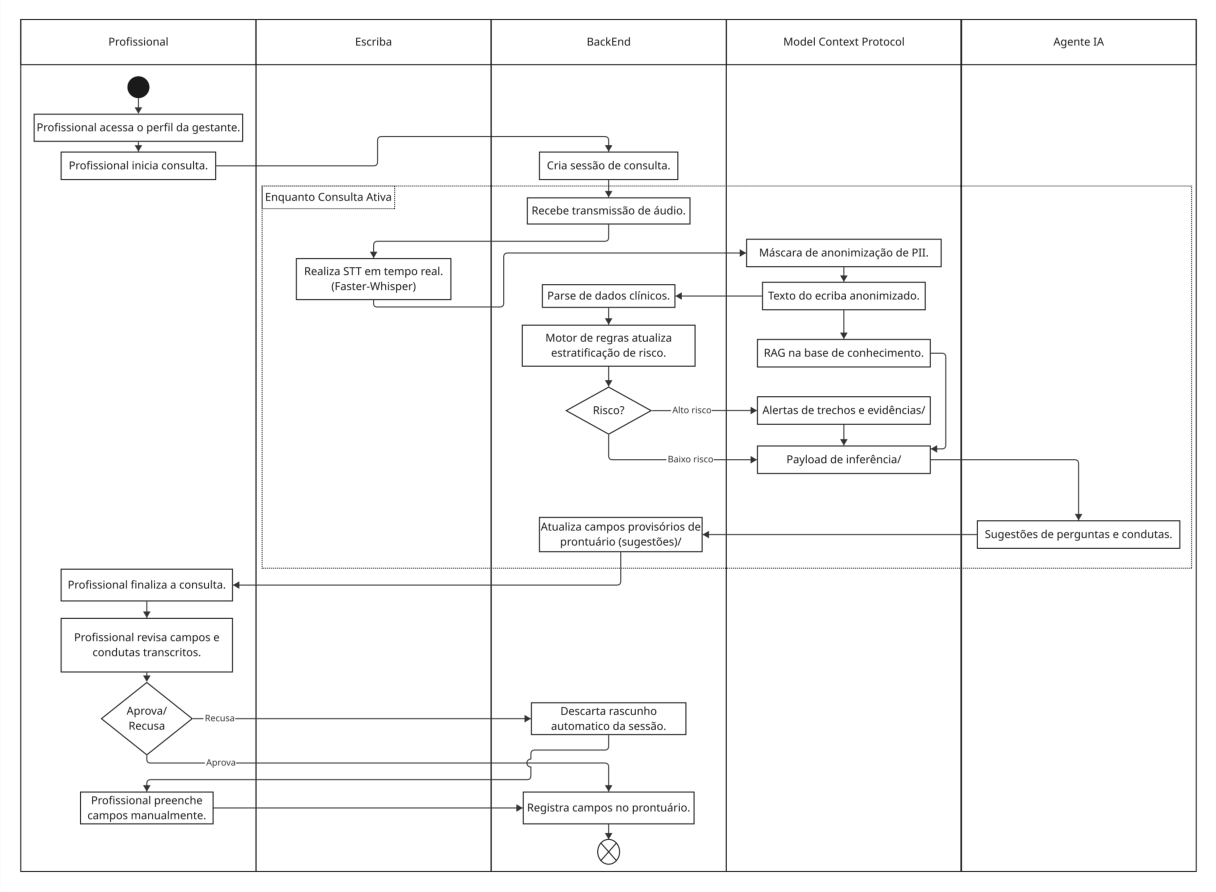
\includegraphics[width=\textwidth, keepaspectratio]{assets/FluxoDeConsulta.pdf}
  \caption{Pipeline arquitetural e ciclo de vida da transação da consulta médica.}
  \label{fig:fluxo_consulta}
\end{figure}

\begin{itemize}
  \item \textbf{Captura e transcrição local (STT):} o fluxo de áudio é transcrito em tempo de execução via \textit{Whisper} com diarização.
  \item \textbf{Sanitização de entrada:} o \textit{gateway} remove ou mascara as \textit{PII} na transcrição antes de compor a consulta ao módulo RAG.
  \item \textbf{Recuperação (Retriever):} a busca retorna os trechos relevantes e aplica MMR para diversificar os \textit{chunks} selecionados e reduzir redundâncias no contexto enviado ao modelo.
  \item \textbf{Geração (Generator):} o LLM sintetiza a resposta clínica com hiperparâmetros conservadores, privilegiando a aderência ao contexto recuperado.
  \item \textbf{Apresentação e validação humana:} a interface exibe as sugestões de preenchimento, mantendo a edição manual integralmente disponível.
\end{itemize}

Para cumprir a restrição de segurança clínica, adota-se uma abordagem baseada no conceito de \textit{Human-in-the-Loop}, onde nenhum dado sugerido pela IA é gravado no banco de dados sem a confirmação explícita do profissional (US04), garantindo o controle total sobre o registro.
A principal ameaça à validade interna é a geração de conteúdo não evidenciado nos protocolos da base de conhecimento, sendo esta mitigada por RAG restrito às diretrizes oficiais e \textit{Human-in-the-Loop}.

A ameaça de exposição de \textit{PII} é mitigada por processamento local em um \textit{gateway} de mascaramento aplicado antes da recuperação e inferência.
O anonimizador foi implementado em arquitetura híbrida, combinando regras determinísticas de Expressões Regulares (RegEx) para identificadores brasileiros e um módulo de Reconhecimento de Entidades Nomeadas (NER) especializado em português biomédico.
Como modelo de NER, utilizou-se \texttt{OpenMed/OpenMed-PII-Portuguese-SnowflakeMed-Large-568M-v1}, disponibilizado no Hugging Face \cite{openmed-pii-2026}.

Na implementação do \textit{gateway}, RegEx cobre e-mail, CPF, CNS, telefones, RG e cadeias numéricas longas, contíguas ou separadas, aplicando \texttt{[EMAIL]}, \texttt{[CPF]}, \texttt{[CNS]}, \texttt{[TELEFONE]} e \texttt{[NUM]}. RegEx e NER geram intervalos mesclados antes da máscara; nomes dependem do NER e, se o \textit{sidecar} falhar, uma heurística de duas a quatro palavras capitalizadas, após remover prefixos como ``Paciente'' e ``Nome'', aplica \texttt{[NOME]}. Assim, o modo \texttt{regex\_only} mantém cobertura determinística de identificadores estruturados.

A modelagem relacional foi derivada da 8ª edição revisada da Caderneta da Gestante, contemplando entidades para paciente, gestação, consultas, sinais vitais, exames, antecedentes, prontuário e registros de atendimento.
O DER completo foi disponibilizado como material suplementar no repositório do projeto.

O módulo de transcrição baseado em Faster-Whisper foi integrado ao protótipo para validar a viabilidade técnica do fluxo de captura local de áudio. Contudo, sua avaliação sistemática não compõe o escopo experimental deste trabalho, permanecendo como etapa futura.

% \begin{figure}[H]
%   \centering
%   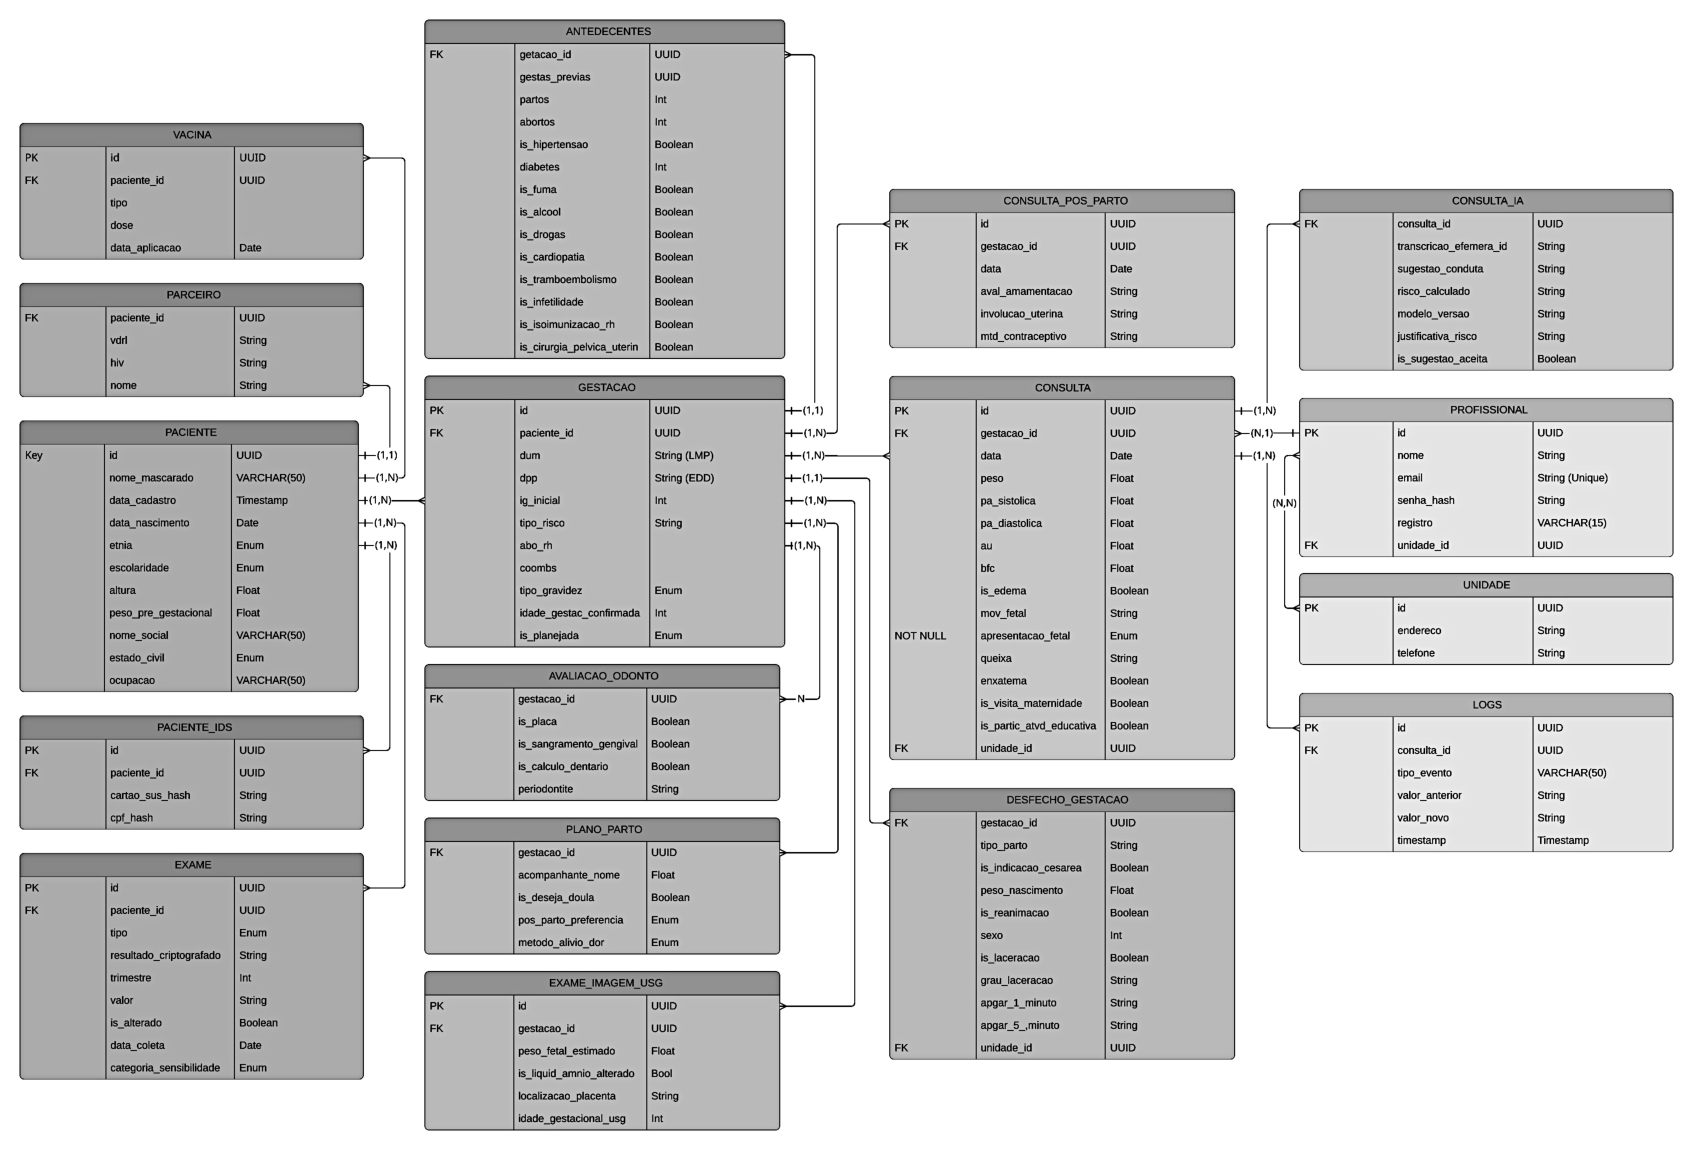
\includegraphics[width=1.1\textwidth, keepaspectratio]{assets/DER_bw.pdf}
%   \caption{Diagrama de Entidade-Relacionamento (DER) do sistema.}
%   \label{fig:der}
% \end{figure}

%%%%%%%%%%%%%%%%%%%%%%%%%%%%%%%%%%%%%%%%%%%%%%%%%%%%%%%%%%%%%%%%%%%%%%%%%%%%%%%%%%%%%%%%%%%%%%%%%%%%%%%%%%%%%%%%%%%%%%%%%%%%%%%%%%%%%%%%%%%%%%%%%%%%%%%%%%%%%%%%%%%%%%

\section{Solução Proposta}

A arquitetura derivou de requisitos funcionais (RF) e histórias de usuário (US) mapeados a riscos clínicos, operacionais e regulatórios.
Para RF03/04, o risco de retenção indevida de áudio é tratado por STT local e descarte do áudio após a transcrição, reduzindo a superfície de vazamento.
RF05 prevê o uso de RAG restrito, system prompts de escopo limitado e guardrails como mecanismos de contenção de respostas fora do domínio. Contudo, a avaliação funcional identificou falha nessa contenção no caso GT05, indicando que esses mecanismos ainda são insuficientes quando utilizados isoladamente.
US04 impede automação indevida: nenhuma sugestão da IA é persistida sem aprovação explícita do profissional, mantendo a decisão final sob sua responsabilidade.
US13 reduz a exposição de PII ao modelo por meio do \textit{gateway} de anonimização, de modo que dados em trânsito chegam mascarados à inferência.
US05 mitiga atraso na identificação de alto risco com alertas determinísticos baseados em limiares das cartilhas, exibidos na interface da consulta.
US06 preserva continuidade do registro físico por exportação em PDF, permitindo uso manual da documentação quando necessário.
As interfaces do protótipo de alta fidelidade, incluindo agenda de atendimentos, prontuário consolidado e tela de consulta ativa com o agente Escriba, foram disponibilizadas como material suplementar no repositório do projeto.
  
% Esses controles foram implementados em um protótipo de alta fidelidade (Figura~\ref{fig:interfaces_compostas}), cobrindo a agenda de atendimentos, o prontuário consolidado da paciente e a tela de consulta ativa com o agente Escriba e o assistente clínico.

% % \begin{figure}[H]
% \begin{figure}[htbp]
%   \centering
%   % --- Primeira Subfigura ---
%   \begin{subfigure}[b]{0.45\textwidth}
%     \centering
%     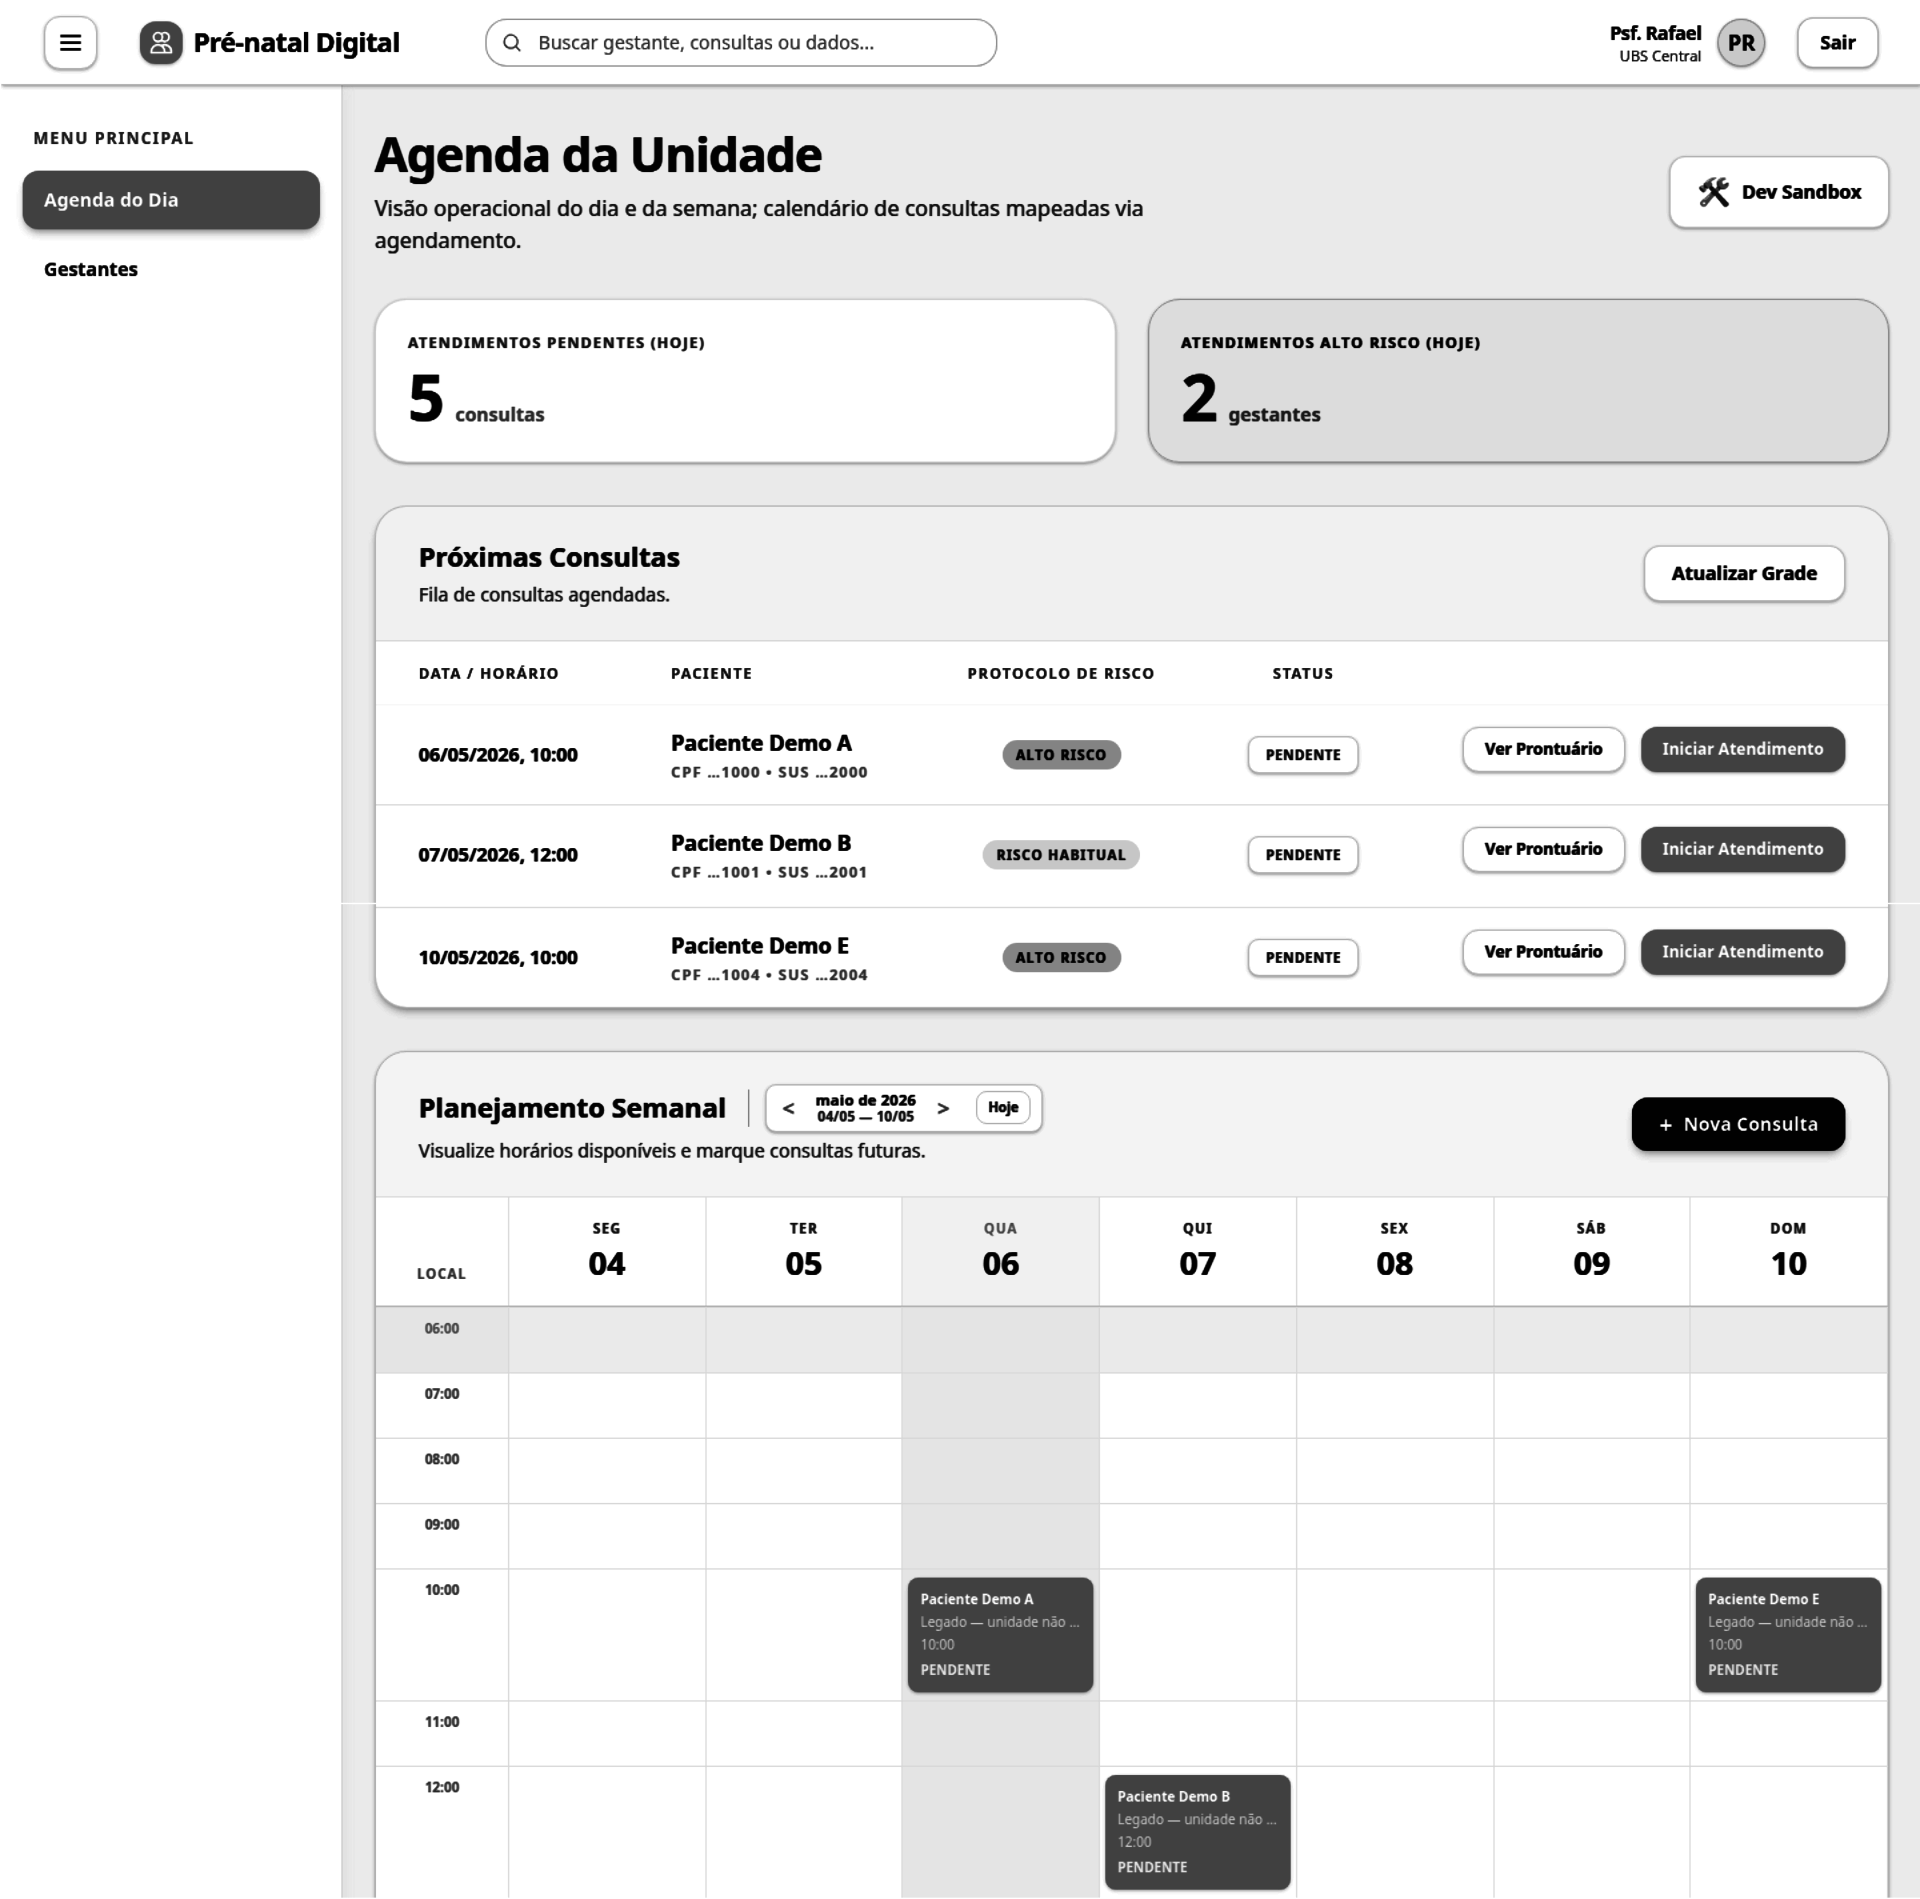
\includegraphics[width=\textwidth, trim={0 0 0 0}, clip]{assets/interfaces/alta_fidelidade/02_dashboard_editted_pb.png}
%     \caption{Painel de gestão (Dashboard).}
%     \label{fig:sub_dashboard}
%   \end{subfigure}
%   \hfill
%   % --- Segunda Subfigura ---
%   \begin{subfigure}[b]{0.50\textwidth}
%     \centering
%     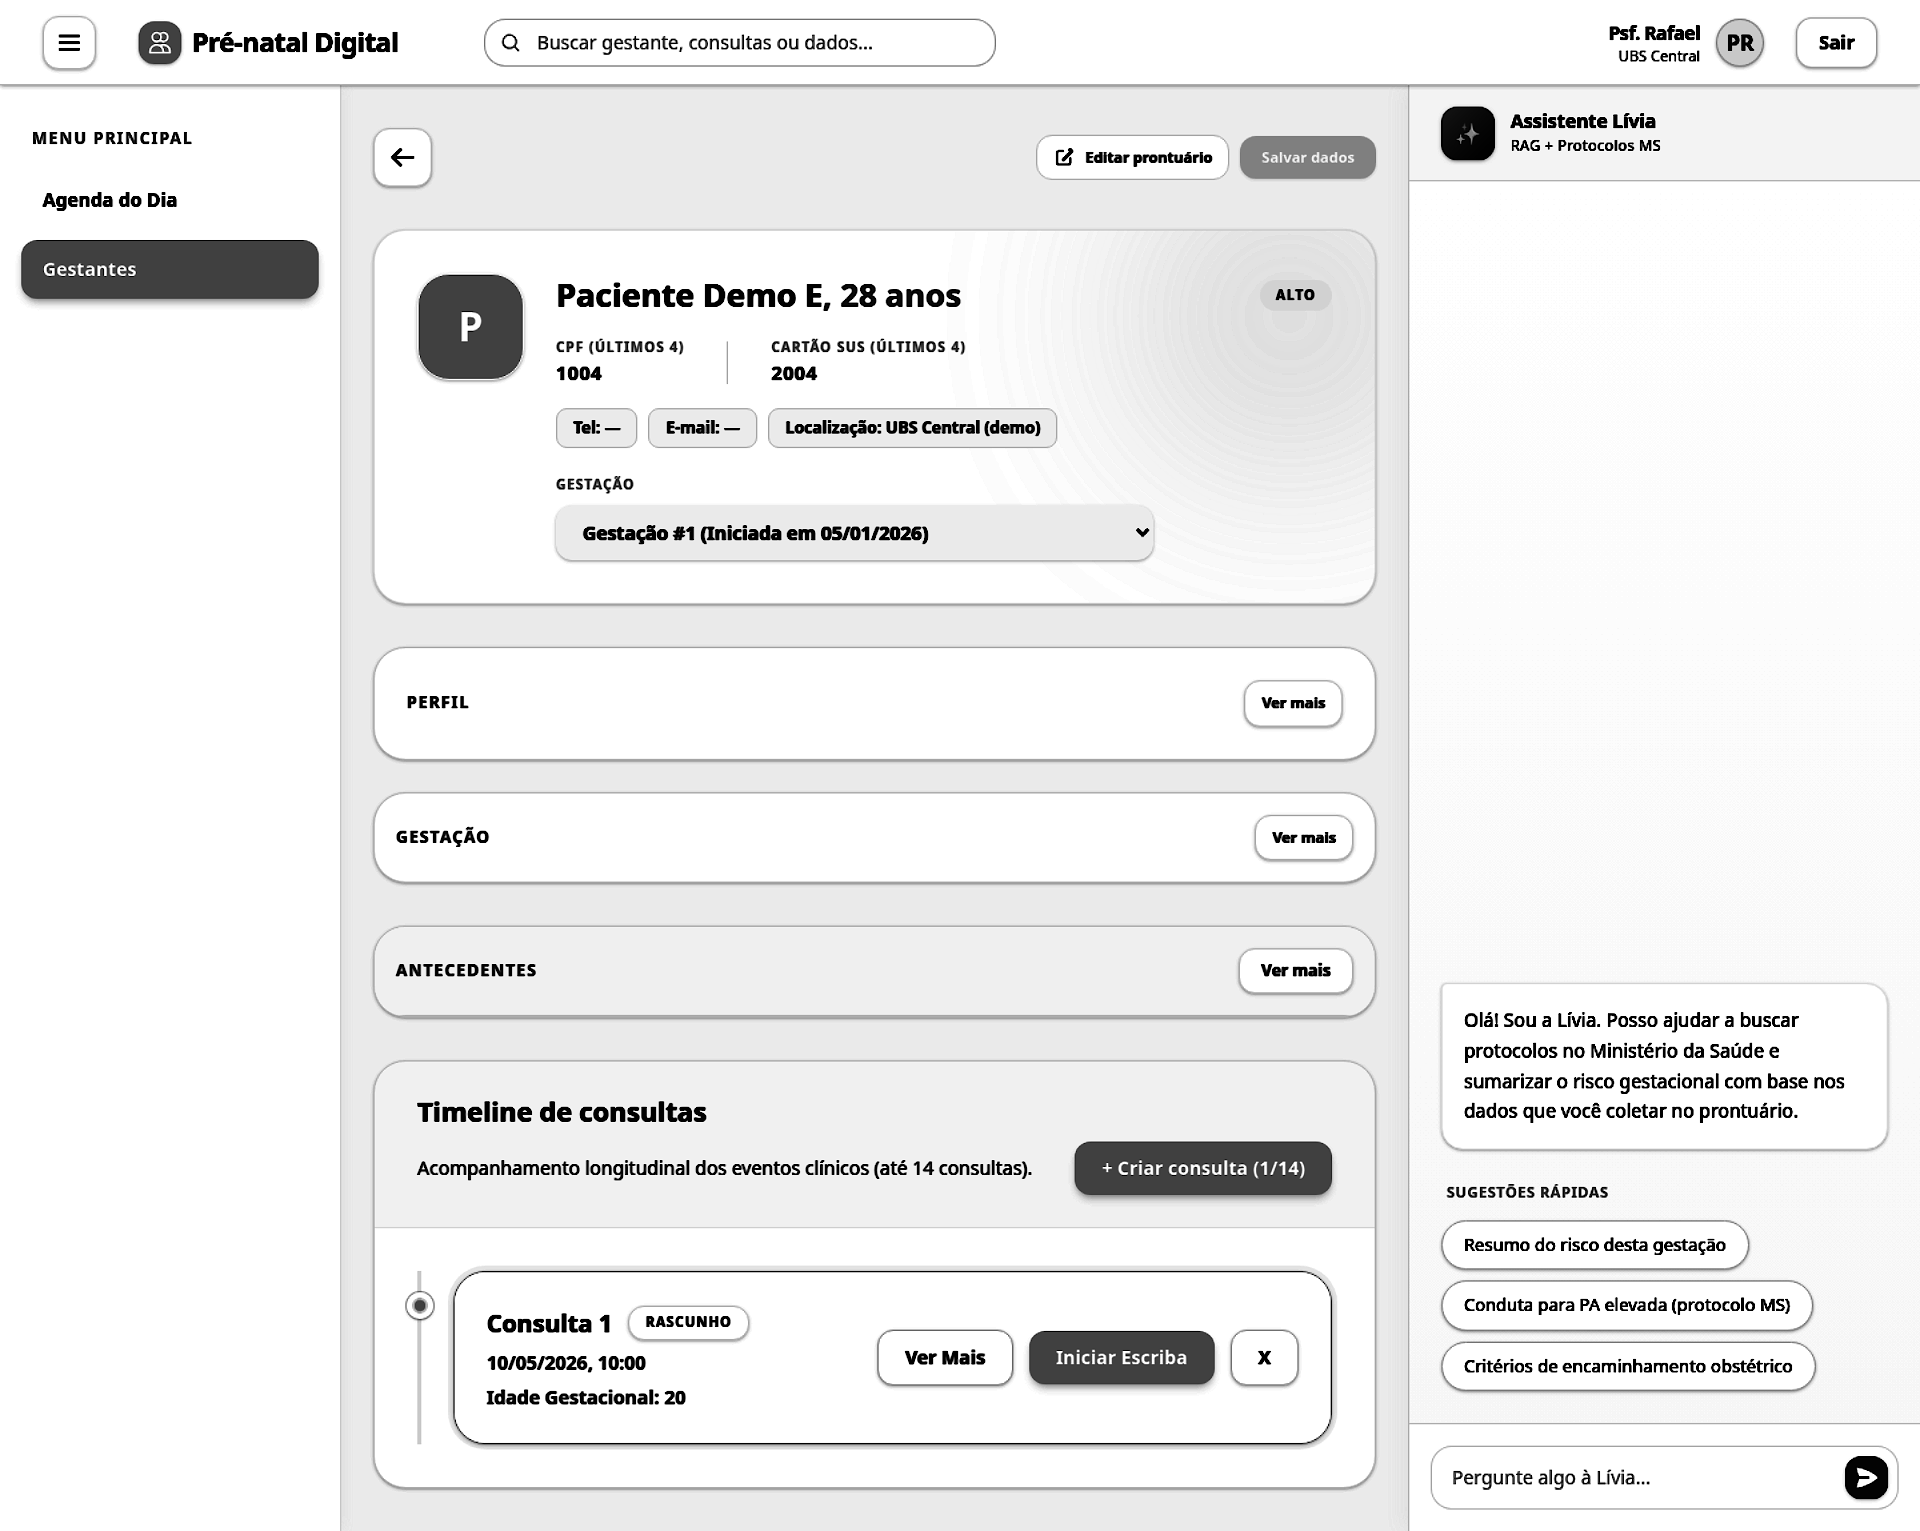
\includegraphics[width=\textwidth, trim={0 0 0 0}, clip]{assets/interfaces/alta_fidelidade/04_paciente_detalhe_pb.png}
%     \caption{Visão consolidada do prontuário.}
%     \label{fig:sub_paciente}
%   \end{subfigure}

%   \vspace{5pt}

%   % --- Terceira Subfigura ---
%   \begin{subfigure}[b]{0.80\textwidth}
%     \centering
%     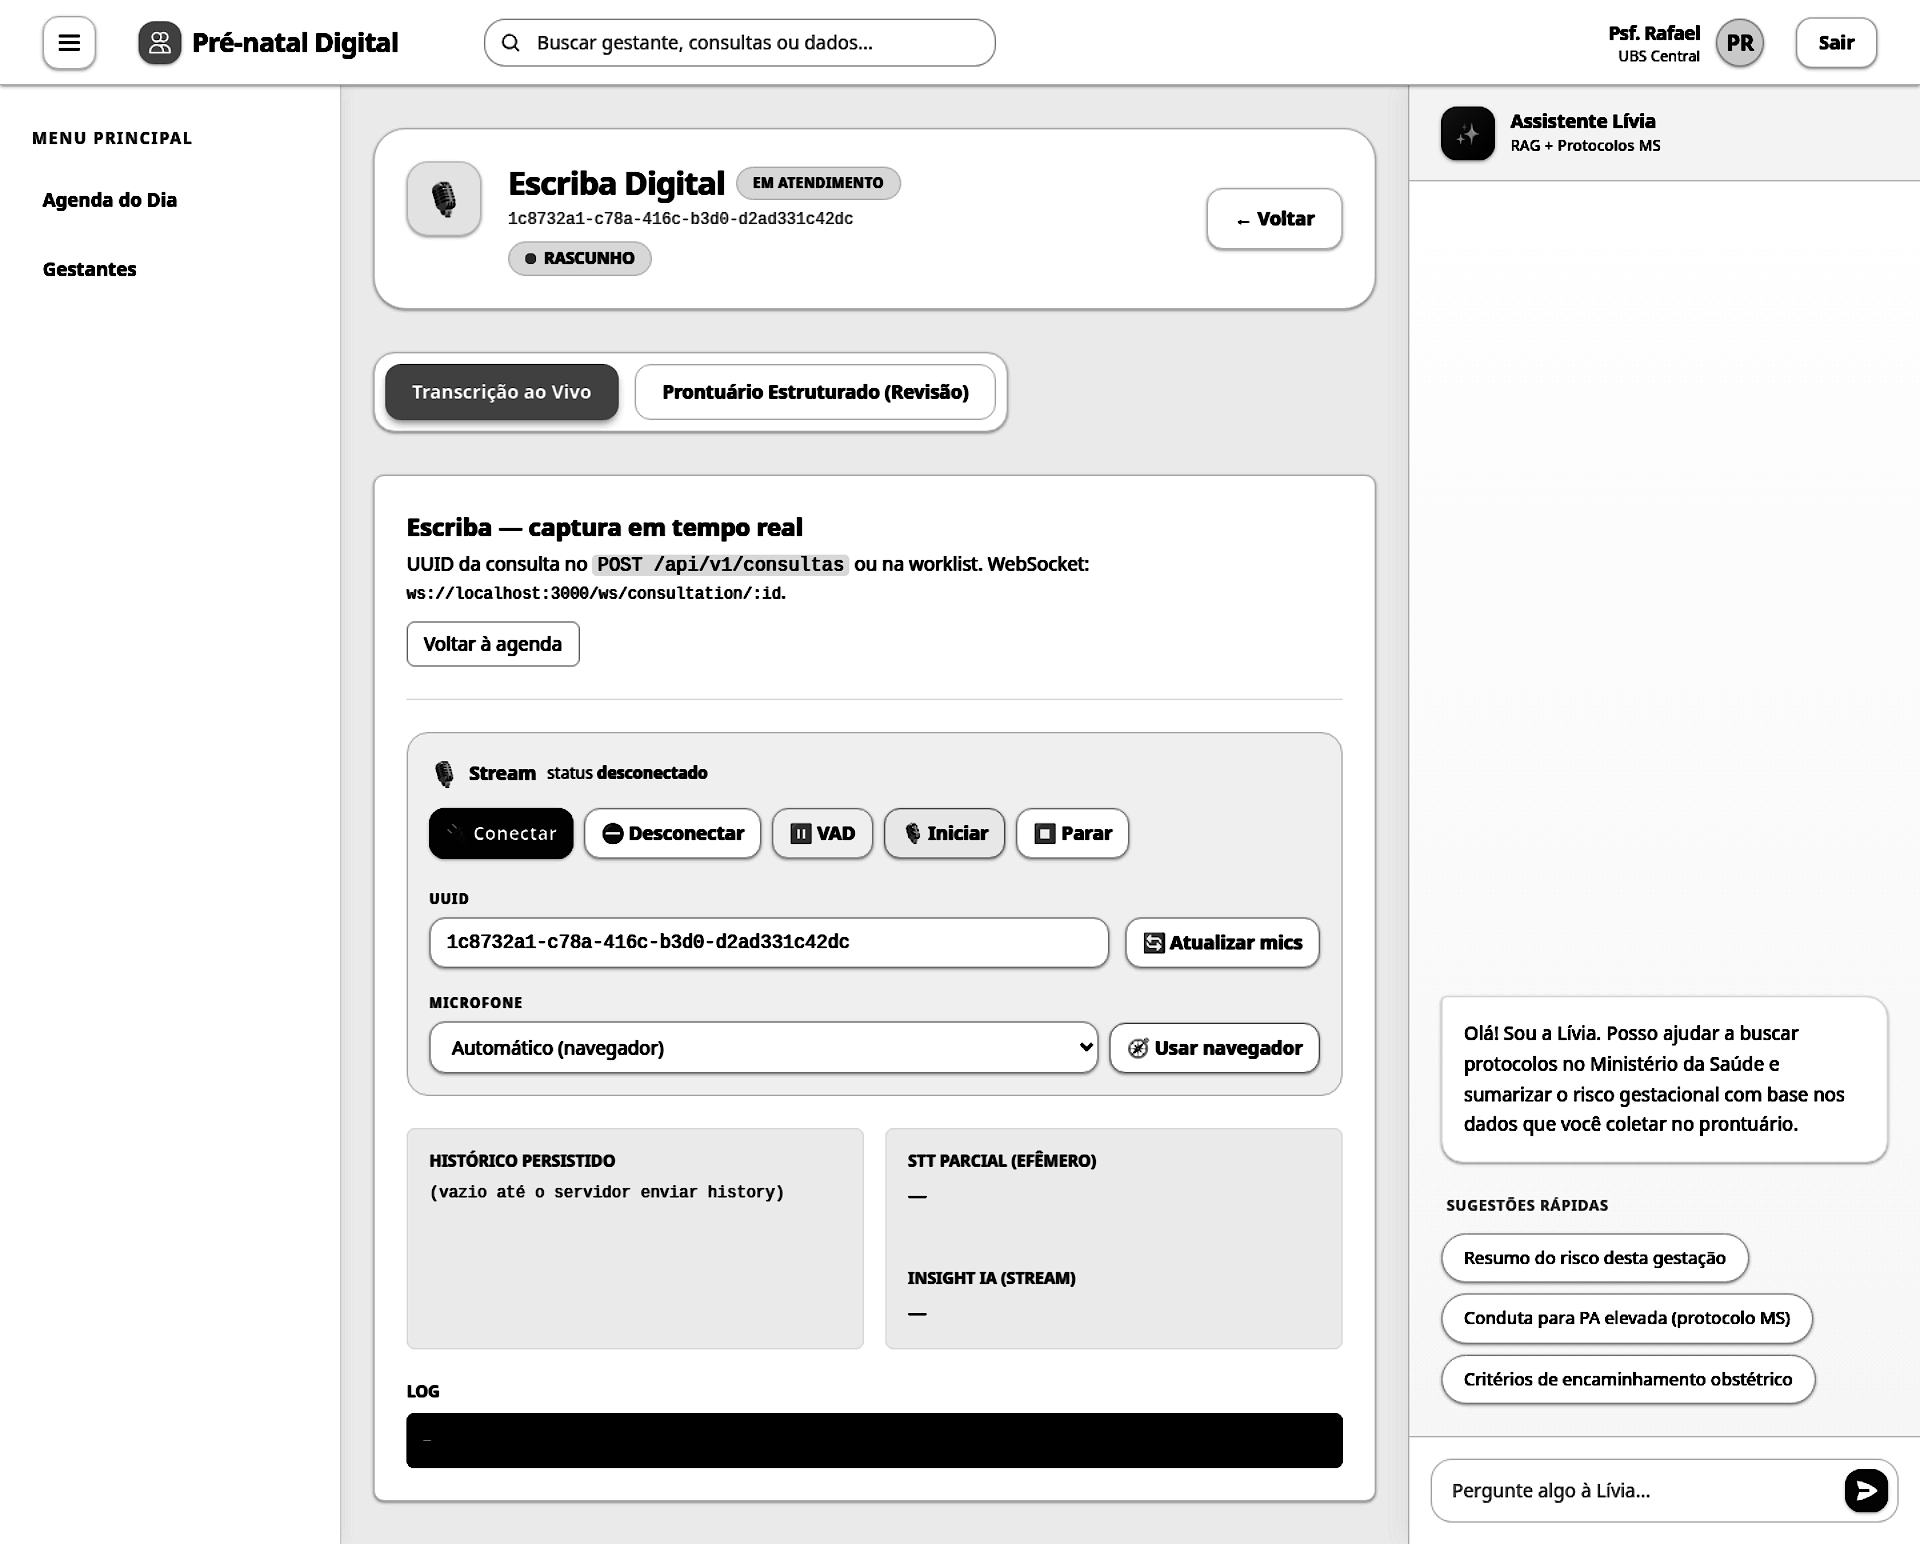
\includegraphics[width=\textwidth, trim={0 0 0 0}, clip]{assets/interfaces/alta_fidelidade/05_escriba_consulta_pb.png}
%     \caption{Interface de atendimento em tempo real.}
%     \label{fig:sub_escriba}
%   \end{subfigure}

%   \caption{Interfaces do protótipo de alta fidelidade: gestão, histórico e atendimento.}
%   \label{fig:interfaces_compostas}
% \end{figure}

%%%%%%%%%%%%%%%%%%%%%%%%%%%%%%%%%%%%%%%%%%%%%%%%%%%%%%%%%%%%%%%%%%%%%%%%%%%%%%%%%%%%%%%%%%%%%%%%%%%%%%%%%%%%%%%%%%%%%%%%%%%%%%%%%%%%%%%%%%%%%%%%%%%%%%%%%%%%%%%%%%%%%%

\section{Avaliação Experimental e Resultados}\label{sec:avaliacao}

A avaliação experimental foi conduzida em três frentes complementares: recuperação documental, geração de respostas e segurança do fluxo clínico. 
O objetivo foi verificar se a arquitetura proposta, baseada em RAG, LLM local e \textit{gateway} de privacidade, consegue recuperar evidências dos manuais oficiais, produzir respostas aderentes aos protocolos e impedir vazamento de informações sensíveis antes da inferência.
O conjunto de testes utilizado contém 100 perguntas em português, das quais 90 avaliam aderência a protocolos e 10 são perguntas distratoras (\textit{trap}).
A distribuição por dificuldade foi de 42 itens fáceis, 35 médios e 23 difíceis.

% Os níveis de dificuldade foram definidos manualmente durante a construção do benchmark.
% Questões fáceis correspondem a consultas diretas cuja resposta pode ser localizada em um único documento ou trecho protocolar.
% Questões de dificuldade média exigem combinar múltiplas informações presentes em diferentes seções de um mesmo manual ou em documentos distintos.
% Questões difíceis envolvem cenários menos frequentes, exceções protocolares ou situações que demandam maior especificidade terminológica para recuperação da evidência correta.

Os níveis de dificuldade foram definidos manualmente durante a construção do benchmark: \textit{easy} abrange consultas diretas localizáveis em um documento ou trecho; \textit{medium}, combinação de seções ou encadeamento de condutas no mesmo manual; e \textit{hard}, cenários menos frequentes, exceções, terminologia específica ou perguntas booleanas armadilhosas. A classificação não foi aprendida automaticamente.

Quatro itens classificados como \texttt{human\_judge} foram mantidos para revisão qualitativa e não compõem o denominador da métrica automática de APR.

% Este sistema de avaliação foi inspirado por práticas da indústria para avaliação de agentes de IA, como as avaliações de agentes do \textit{Microsoft Copilot Studio} \cite{MicrosoftCopilotEval2026}.

Um item é \textit{trap} quando \texttt{notes\_scoring\_pt} contém \texttt{tag=trap}; na TFR, \texttt{boolean\_exact} requer a primeira resposta SIM/NÃO igual ao gabarito e ausência de \texttt{must\_not\_contain\_pt}; resposta incorreta ou conteúdo proibido é falha. Como exemplo, Q013 pergunta se a azitromicina substitui a penicilina para tratar sífilis na gestante: a resposta esperada é NÃO, e ``azitromicina substitui'' ou ``eritromicina cura'' são proibidas.

%---------------------------------------------------------------------------------------------------------------------------------------------------------------------

\subsection{Recuperação Semântica}

O módulo de recuperação foi avaliado isoladamente com \textit{top-k}=6 e expansão de consulta ativada.
O valor de $k$ foi definido como escolha operacional intermediária, buscando equilibrar cobertura documental e controle de ruído no contexto enviado ao modelo.
Foram utilizadas três métricas:
\textit{Hit@6}, que verifica se o documento-fonte esperado aparece entre os seis primeiros \textit{chunks};
\textit{Mean Reciprocal Rank} (MRR), que mede quão cedo o primeiro documento correto aparece na lista recuperada. Quanto mais próximo da primeira posição estiver o documento esperado, maior será o valor da métrica, aproximando-se de 1;
e \textit{phrase\_recall}, que mede a presença das frases esperadas nos trechos recuperados.
Além de apoiar a geração de respostas, o RAG acrescenta uma camada de rastreabilidade documental ao sistema, pois permite associar cada resposta aos trechos recuperados, seus documentos de origem e respectivos metadados.
Essa característica aumenta a auditabilidade das respostas e favorece a revisão humana, aspecto relevante em sistemas de apoio informacional no contexto médico.
A Tabela~\ref{tab:metricas_rag} apresenta os resultados por dificuldade.


\begin{table}[H]
  \centering
  \caption{Desempenho do módulo RAG por nível de dificuldade ($n=100$).}
  \label{tab:metricas_rag}
  \small
  \begin{tabular}{lccc}
  	\toprule
  	\textbf{Dificuldade} & \textbf{n}   & \textbf{Hit@6 (\%)}  & \textbf{MRR Médio} \\
  	\midrule
  	Easy                 & 42           & 76,2\%               & 0,4837             \\
  	Medium               & 35           & 68,6\%               & 0,3633             \\
  	Hard                 & 23           & 95,7\%               & 0,6536             \\
  	\midrule
  	\textbf{Global}      & \textbf{100} & \textbf{78,0\%}      & \textbf{0,4807}    \\
  	\bottomrule
  	\end{tabular}
  \end{table}
  
O \textit{phrase\_recall} médio global foi de 47,1\%.
Embora os casos encontrados nos itens difíceis representem situações potencialmente mais complexas do ponto de vista clínico, eles frequentemente utilizam terminologia mais específica e menos ambígua, o que favorece a recuperação vetorial.
Em contraste, perguntas rotineiras de pré-natal apresentam maior sobreposição semântica entre documentos, aumentando a competição entre trechos similares durante o ranqueamento.

%---------------------------------------------------------------------------------------------------------------------------------------------------------------------

\subsection{Geração de Resposta}

A geração foi avaliada por meio da Taxa de Aprovação de Respostas (APR) correspondente à proporção de frases obrigatórias aprovadas segundo os critérios de protocolo, calculada sobre itens elegíveis à avaliação automática, e da Taxa de Falha em Perguntas Distratoras (TFR), calculada sobre os itens \textit{trap}.
O modelo local Qwen3.5 9B foi executado com e sem RAG para medir o ganho incremental da recuperação.
O Gemini-3.1-Flash-Lite foi utilizado apenas como linha de base externa de comparação, recebendo o mesmo contexto recuperado pelo RAG do protótipo, mas sem integrar a arquitetura \textit{on-premise} proposta.

\begin{table}[H]
  \centering
  \caption{Desempenho dos modelos na geração de respostas.}
  \label{tab:apr_tfr_providers}
  \small
  \begin{tabular}{lccc}
  	\toprule
  	\textbf{Provedor}           & \textbf{Modo RAG} & \textbf{APR (\%)} & \textbf{TFR (\%)} \\
  	\midrule
  	Qwen3.5 9B (Ollama)         & Off               & 53,1\% (51/96)    & 20,0\% (2/10)     \\
	  Qwen3.5 9B (Ollama)         & On                & 57,3\% (55/96)    & 10,0\% (1/10)     \\
  	Gemini-3.1-Flash-Lite       & On                & 61,5\% (59/96)    & 0\% (0/10)      \\
  	\bottomrule
  \end{tabular}
  \end{table}

A ativação do RAG no modelo local elevou a APR de 53,1\% para 57,3\% e reduziu a TFR de 20,0\% para 10,0\%.
O ganho é limitado, indicando que a recuperação documental contribui para reduzir respostas inseguras, mas não garante aderência clínica estrita quando o modelo precisa negar condutas, reproduzir termos literais ou resolver conflitos entre documentos.
No conjunto total de execuções, foram registradas 3 falhas em itens \textit{trap} e 120 reprovações de protocolo nas 258 avaliações automáticas de frases obrigatórias.
Os quatro itens excluídos da avaliação demandam revisão qualitativa da equipe clínica e não entram no denominador da Tabela~\ref{tab:apr_tfr_providers}.

%---------------------------------------------------------------------------------------------------------------------------------------------------------------------

\subsection{Privacidade, escopo e latência}

O módulo de anonimização foi submetido a 50 frases sintéticas, totalizando 76 entidades sensíveis avaliadas, incluindo CPF, Cartão Nacional de Saúde (CNS), e-mail, telefone, nomes completos e cadeias numéricas longas.
Não houve vazamento detectado no conjunto testado, conforme a Tabela~\ref{tab:pii_leak}. Esse resultado valida a implementação inicial do mascaramento, mas não elimina a necessidade de testes com variações linguísticas, abreviações e ruído de transcrição.

\begin{table}[H]
  \centering
  \caption{Taxa de vazamento de PII por tipo de entidade.}
  \label{tab:pii_leak}
  \small
  \begin{tabular}{lcc}
  	\toprule
	\textbf{Entidade} 	 	                & \textbf{n} 		                & \textbf{Leak Rate (\%)} \\
	\midrule
  	CNS     			                      & 11                            & 0\%                   \\
  	CPF                                 & 12                            & 0\%                   \\
  	E-mail                              & 12                            & 0\%                   \\
  	Nome Completo			                  & 21                            & 0\%                   \\
  	Cadeias Numéricas Longas            & 8                             & 0\%                   \\
  	Telefone                            & 12                            & 0\%                   \\
	\midrule
  	\textbf{Total Global}               & \textbf{76}                   & \textbf{0\%}          \\
  	\bottomrule
  \end{tabular}
  \end{table}
 
Além das métricas agregadas, aplicou-se o roteiro funcional (GT01-GT05), composto por cinco casos sintéticos para validar comportamentos essenciais do protótipo.
Os casos GT01, GT02 e GT03 avaliam respostas clínicas com RAG e LLM em cenários de risco alto extraídos dos manuais protocolares.
O GT04 avalia sanitização direta de PII.
O GT05 avalia a capacidade de recusar uma requisição fora do escopo de pré-natal.

O roteiro funcional obteve sucesso em quatro dos cinco casos avaliados.
Os três casos clínicos com RAG e LLM foram aprovados, assim como o caso de sanitização direta de PII.
A falha ocorreu no GT05, no qual a barreira de escopo não conteve adequadamente uma requisição fora do domínio pré-natal.
Esse resultado indica que a segurança comportamental não deve depender apenas de \textit{system prompts} e o módulo de privacidade deve incorporar verificações determinísticas ou classificadores de escopo antes da síntese pelo modelo.

Quanto à eficiência computacional, as métricas foram segregadas por configuração para evitar que a linha de base em nuvem distorça a interpretação operacional do protótipo local. A Tabela~\ref{tab:latencia_config} apresenta os resultados médios.

\begin{table}[H]
  \centering
  \caption{Latência média por configuração de execução.}
  \label{tab:latencia_config}
  \small
  \begin{tabular}{lrrrr}
    \toprule
    \textbf{Configuração} 		& \textbf{Retrieve (ms)} 	& \textbf{Latência total (s)} 	& \textbf{TTFT (ms)} 	& \textbf{tokens/s} \\
    \midrule
    Qwen3.5 9B (Ollama)			& --    		 	& 11,71 			& 470,1  		& 32,5 \\
    Qwen3.5 9B (Ollama)   + RAG on  	& 373,1 			& 15,59 			& 2789,7 		& 32,4 \\
    Gemini-3.1-Flash-Lite + RAG on 	& 372,7 			& 4,55  			& 3501,9 		& 360,6 \\
    \bottomrule
  \end{tabular}
\end{table}

Para o protótipo local, a recuperação vetorial acrescentou aproximadamente 373 ms ao fluxo, enquanto a latência total do Qwen3.5 9B com RAG foi de 15,59 segundos.
Portanto, o gargalo operacional permanece na inferência local do LLM e no aumento de contexto provocado pelo RAG, não na busca vetorial.
A linha de base externa apresentou maior vazão de geração, mas não representa a premissa de privacidade local da arquitetura proposta.
Esse resultado reforça que a adoção em produção de baixo custo ainda é limitada pelos requisitos de hardware, especialmente VRAM, tempo de inferência e estabilidade sob carga.

%%%%%%%%%%%%%%%%%%%%%%%%%%%%%%%%%%%%%%%%%%%%%%%%%%%%%%%%%%%%%%%%%%%%%%%%%%%%%%%%%%%%%%%%%%%%%%%%%%%%%%%%%%%%%%%%%%%%%%%%%%%%%%%%%%%%%%%%%%%%%%%%%%%%%%%%%%%%%%%%%%%%%%

\section{Discussão}\label{sec:discussao}
Os resultados indicam viabilidade técnica parcial da arquitetura proposta.
A combinação de execução local, RAG restrito a documentos oficiais e mascaramento de PII atende ao objetivo de reduzir dependência de nuvem pública e de oferecer um fluxo mais controlável do ponto de vista da LGPD.
Os resultados mostram que o protótipo ainda não pode ser interpretado como sistema autônomo de apoio clínico; ele foi concebido como ferramenta assistiva e documental.
A APR do modelo local com RAG foi de 57,3\%, e a TFR permaneceu em 10,0\%; portanto, a recuperação documental melhora o comportamento do LLM, mas não elimina erros em respostas que exigem negação explícita, fidelidade literal ou distinção entre protocolos semanticamente próximos.

% O desempenho do RAG ajuda a explicar esse limite, onde o \textit{Hit@6} global de 78,0\% demonstre boa capacidade de recuperar ao menos um documento relevante entre os seis primeiros trechos, o \textit{phrase\_recall} médio de 47,1\% indica que a evidência recuperada nem sempre contém as frases necessárias para satisfazer o critério de resposta.
O desempenho do RAG com \textit{Hit@6} global de 78,0\% demonstra boa capacidade de recuperar ao menos um documento relevante entre os seis primeiros trechos; o \textit{phrase\_recall} médio de 47,1\% indica que a evidência recuperada nem sempre contém as frases necessárias para satisfazer o critério de resposta.
Ou seja, o modelo tende a receber um documento correto, mas sem o trecho suficientemente específico para responder com segurança.
% Esse comportamento é compatível com a assimetria observada por dificuldade: itens difíceis, frequentemente associados a termos técnicos de alto risco, foram mais bem recuperados do que itens médios, nos quais há maior competição lexical entre manuais de pré-natal de rotina.

Na análise complementar por dificuldade, que agrega execuções Ollama com RAG ativado e desativado, a APR foi maior em \textit{hard} (72,5\%) do que em \textit{easy} (48,8\%) e \textit{medium} (52,9\%). A mesma hierarquia aparece na recuperação: \textit{hard} obteve Hit@6 de 95,7\% e MRR de 0,6536, acima de \textit{easy} (76,2\%; 0,4837) e \textit{medium} (68,6\%; 0,3633), sugerindo convergência entre recuperação e geração. O menor resultado em \textit{medium} é compatível com competição semântica em perguntas rotineiras, e não implica ausência de utilidade global do recuperador. Por agregar os dois modos, essa APR não isola o efeito do RAG nem substitui a APR de 57,3\% com RAG ativado da Tabela~\ref{tab:apr_tfr_providers}. Dos 23 itens \textit{hard}, 10 são \textit{trap}, o que influencia a geração nesse estrato; o Hit@6 elevado, porém, avalia todas as perguntas classificadas como difíceis.

No desenho do benchmark, itens \textit{easy} e \textit{medium} correspondem majoritariamente a consultas diretas ou encadeamentos de rotina presentes nos protocolos de baixo risco; para profissionais familiarizados com esses fluxos, a busca documental adicional pode ter valor marginal menor. Já os itens \textit{hard} concentram exceções, terminologia de alto risco e condutas menos frequentes descritas nos manuais específicos. \cite{ManualAltoRisco2022} Assim, a convergência observada em \textit{hard} sugere que o protótipo pode se alinhar melhor a um papel assistivo em dúvidas pontuais de maior especificidade, desde que a evidência recuperada permaneça sujeita à revisão humana. Como hipótese de desenho, a latência de aproximadamente 15,59~s com RAG (Tabela~\ref{tab:latencia_config}) pode representar relação custo-benefício informacional mais favorável nessas consultas do que em demandas rotineiras repetitivas; essa preferência não foi medida com usuários.

Em especial, nos itens classificados como difíceis, o módulo RAG atingiu Hit@6 de 95,7\% e MRR de 0,6536, sugerindo maior efetividade em cenários com terminologia protocolar mais específica.

A comparação com o Gemini cria uma nova perspectiva quanto à falha da solução local.
O modelo externo atingiu APR superior e TFR nula sob a mesma configuração de RAG, sugerindo que o recuperador atual pode sustentar respostas melhores quando acoplado a modelos mais capazes.
O resultado aponta, portanto, para a necessidade de avaliar modelos locais maiores ou melhor adaptados a terminologia clínica, desde que acompanhados de hardware compatível e controles de privacidade equivalentes.

% O resultado de 0,0\% de vazamento de PII no corpus sintético é positivo, mas sua validade externa é limitada. Nomes brasileiros compostos, abreviações, fala espontânea, erros de transcrição e regionalismos podem gerar padrões fora da distribuição testada. Como o módulo STT não foi avaliado sistematicamente, a transcrição é tratada como dado sensível em trânsito e como pré-preenchimento editável. Essa limitação reforça o papel do fluxo \textit{human-in-the-loop}: o profissional deve validar tanto a informação clínica quanto a integridade dos dados inseridos antes da persistência.
A ausência de vazamentos de PII no corpus sintético é um resultado positivo, mas sua validade externa é limitada. Nomes brasileiros compostos, abreviações, fala espontânea, erros de transcrição e regionalismos podem gerar padrões fora da distribuição testada.
Como o módulo STT não foi avaliado sistematicamente, a transcrição é tratada como dado sensível em trânsito e como pré-preenchimento editável.
Essa limitação reforça o papel do fluxo \textit{human-in-the-loop}: o profissional deve validar tanto a informação clínica quanto a integridade dos dados inseridos antes da persistência.

As limitações do estudo decorrem do próprio escopo experimental.
A avaliação realizada mede viabilidade arquitetural, privacidade, recuperação documental, aderência automática e comportamento funcional em casos sintéticos; ela não mede eficácia assistencial. Não houve avaliação com gestantes, profissionais de saúde ou dados clínicos reais, logo, os resultados não permitem inferir redução efetiva de carga cognitiva, usabilidade em consulta ou impacto sobre desfechos de cuidado.
Além disso, o agente escriba e o módulo STT foram validados apenas quanto à integração funcional ao protótipo, sem métricas formais de qualidade de transcrição, latência ou robustez em ambientes clínicos.

Como trabalhos futuros, recomenda-se refinar a indexação por metadados de versão dos manuais, implementar barreiras determinísticas de escopo antes da geração, avaliar sistematicamente o módulo de transcrição em áudio clínico simulado, comparar modelos locais maiores ou ajustados ao domínio médico e validar o protótipo com profissionais de saúde mediante aprovação ética.
Também devem ser mensurados consumo de VRAM, latência e estabilidade sob carga em diferentes configurações de hardware.


%%%%%%%%%%%%%%%%%%%%%%%%%%%%%%%%%%%%%%%%%%%%%%%%%%%%%%%%%%%%%%%%%%%%%%%%%%%%%%%%%%%%%%%%%%%%%%%%%%%%%%%%%%%%%%%%%%%%%%%%%%%%%%%%%%%%%%%%%%%%%%%%%%%%%%%%%%%%%%%%%%%%%%

\section{Conclusão}\label{sec:conc}

Este trabalho especificou, implementou e avaliou um sistema protótipo \textit{on-premise} para apoio documental ao pré-natal no contexto do SUS, integrando transcrição local, RAG sobre manuais oficiais, LLM executado via Ollama com revisão humana obrigatória e um \textit{gateway} de anonimização de dados.

A pergunta norteadora foi respondida de forma parcial:
a arquitetura mostrou-se tecnicamente viável como base assistiva, auditável e não autônoma, mas os resultados de geração, escopo e latência indicam que o sistema ainda não possui robustez suficiente para uso clínico sem supervisão profissional.
A topologia em contêineres deve ser entendida como decisão de privacidade por desenho, não como comprovação de isolamento absoluto, pois não foram realizados testes específicos de segurança de rede.

Na avaliação experimental, o módulo \textit{RAG} alcançou \textit{Hit@6} global de 78,0\% e MRR médio de 0,4807, com \textit{phrase\_recall} médio de 47,1\%, indicando capacidade razoável de recuperar documentos relevantes, embora a evidência recuperada nem sempre contenha o trecho necessário para satisfazer integralmente o critério de resposta.
O resultado mais expressivo foi observado nos itens classificados como difíceis, para os quais o módulo RAG atingiu Hit@6 de 95,7\%, sugerindo potencial utilidade em cenários menos rotineiros e com maior especificidade protocolar.

O módulo de privacidade não apresentou vazamento no conjunto sintético de 76 entidades avaliadas, embora esse resultado não substitua testes com fala espontânea, abreviações, erros de transcrição e maior variação linguística.
A latência média de 15,59 segundos no fluxo local com \textit{RAG} evidencia que a inferência local e os requisitos de hardware ainda limitam a adoção de baixo custo em produção.
Por fim, a revisão humana obrigatória foi validada como restrição de projeto, pois os resultados reforçam que o sistema deve permanecer assistivo, auditável e não autônomo.
A aprovação de quatro dos cinco casos funcionais do roteiro (GT01-GT05) indica coerência funcional inicial, enquanto a falha no GT05 evidencia a necessidade de barreiras de escopo antes da geração via \textit{LLM}.

%Em relação aos objetivos,
%o trabalho cumpriu a revisão conceitual sobre IA Responsável, privacidade e LLMs;
%rojetou uma arquitetura local em contêineres;
%implementou um protótipo funcional com RAG, LLM local, mascaramento de PII e revisão humana obrigatória;
%estruturou um benchmark reprodutível de recuperação e geração;
%e avaliou o sistema por métricas de recuperação, aderência automática, PII sintética, escopo e latência.
%Entretanto, a avaliação não mediu impacto assistencial, usabilidade em consulta, redução de carga cognitiva ou desempenho com dados reais

Como contribuição, o estudo entrega uma arquitetura replicável, um fluxo de privacidade alinhado aos princípios da LGPD e um benchmark inicial reprodutível para avaliação técnica de recuperação, geração, mascaramento de PII, escopo e latência em documentos de pré-natal.
Os resultados evidenciam os trade-offs entre execução local, custo computacional e segurança operacional, indicando que avanços em modelos, quantização, aceleração em hardware e técnicas de RAG podem tornar esse tipo de sistema mais viável em ambientes reais.

%%%%%%%%%%%%%%%%%%%%%%%%%%%%%%%%%%%%%%%%%%%%%%%%%%%%%%%%%%%%%%%%%%%%%%%%%%%%%%%%%%%%%%%%%%%%%%%%%%%%%%%%%%%%%%%%%%%%%%%%%%%%%%%%%%%%%%%%%%%%%%%%%%%%%%%%%%%%%%%%%%%%%%

\section{Declarações Finais}

% Os materiais suplementares estão disponíveis no repositório público do projeto: \url{https://github.com/lucaszegrine/sus-prenatal-ai-icei-puc-minas-cc}.

Os materiais suplementares estão disponíveis no repositório público do projeto: \href{https://github.com/lucaszegrine/sus-prenatal-ai-icei-puc-minas-cc}{//github.com/lucaszegrine/sus-prenatal-ai-icei-puc-minas-cc}.

O estudo não envolve participantes humanos, não utiliza dados clínicos reais identificáveis e não foi submetido ao Comitê de Ética em Pesquisa da PUC Minas. 

Durante a preparação do texto, foi utilizado o modelo Gemini 3.1 Pro (Google, 04/2026) para revisão gramatical e refinamento de clareza.
A ferramenta não foi utilizada para geração de resultados experimentais, análise de resultados ou compartilhamento de dados sensíveis.
Todo o conteúdo obtido de forma automatizada foi revisado e editado conforme necessário, sob total responsabilidade dos autores.

% \section{Comitê de Ética:}
% O estudo não envolve participantes humanos e não foi submetido ao Comitê de Ética em Pesquisa da PUC Minas.

% \section{Funding e suporte:}
% Esse trabalho não recebeu nenhum tipo de financiamento ou suporte financeiro.

% \section{Conflitos de interesse:}
% Não há conflitos de interesse.

% \section{Declaração de uso de Inteligência Artificial:}
% Durante a preparação deste trabalho, o autor utilizou o modelo de linguagem de grande escala Gemini 3.1 Pro (Google, 04/2026) para revisão gramatical e refinamento de clareza textual onde todo o conteúdo obtido de forma automatizada foi revisado e editado conforme necessário sob total responsabilidade do autor.
% A ferramenta não foi utilizada para geração de resultados experimentais ou análise de resultados assim como nenhum dado sensível ou identificável foi compartilhado com a ferramenta.

\newpage

\bibliographystyle{sbc}
% \bibliography{sbc-template}
\bibliography{sbc}

\end{document}